\section{X線・原子核と原子核反応}

% ===========================================================================
%  再編（2026-09-24）：第5章 原子物理 の第34回（原子の最終回・全体の最終回）．
%  原本の 第45回「X線・放射壊変」の 45.2 以降（45.1 は第33回）と 第46回「原子核反応」の全体を1回にまとめ，
%  原子物理の章末問題 [24][25] を加えた（章末 [23] は電磁気の第29回へ移してある）．
%
%  ・練習は13題．練習番号は第33回（［1］〜［9］）の続き（\setcounter{qno}{9}）．
%      A問題 ［10］＝㊻[17]（基本事項の確認）
%      B問題 ［11］＝㊺[12]（X線の発生機構）  ［12］＝㊺[13]（ブラッグ反射条件・物質波・指定）
%            ［13］＝㊺[14]（放射壊変・指定）  ［14］＝㊺[15]（放射壊変の回数）  ［15］＝㊻[18]（半減期）
%            ［16］＝㊻[19]（原子核反応式）  ［17］＝㊻[20]（結合エネルギー・指定）  ［18］＝㊻[21]（炭素14・指定）
%      C問題 ［19］＝㊺[16]（物質波の波長）  ［20］＝㊻[22]（原子核反応）
%            ［21］＝㊻章末[24]（α粒子と原子核）  ［22］＝㊻章末[25]（質量とエネルギー）
%    再編案の表は第34回を「12題」としているが，［12］〜［22］の11題＋章末2題で13題になる（第33回の注を参照）．
%
%  ・例題は7題．第33回が【例題1】〜【例題7】なので \setcounter{nombre}{7} として【例題8】〜【例題14】．
%    原本の例題8〜14 をそのまま使った（理想の4題より多いが，いずれも小問1〜3個の確認問題で節ごとに1題ずつ）．
%
%  ・【重要】原本の講義編（例題を含む）は Google Drive の OCR テキストしか取れなかった．
%    本文は physics_ch45〜46.tex の打ち込みを使い，例題の問題文は OCR から復元した．要照合：
%      ・例題8：加速電圧 60 kV，横軸 ×10^{-11} m（目盛 5・10）までは OCR の通り．**グラフの形（特性X線の位置）は再構成**．
%      ・例題9：表の質量数（224・226・228・228・228・232・234）と核外電子数（88・88・88・89・90・90・90），
%        原子番号 88・89・90 が Ra・Ac・Th であることは OCR の通り．設問 (1)〜(3) も OCR の通り．
%      ・例題10：「U が自然放射を繰り返して最終的に Pb」は OCR の通りだが，**質量数（238→206）は再構成**（ウラン系列）．
%      ・例題11：${}^{226}$Ra，半減期 1622 年，(1) 1/16 (2) 3244 年前 は OCR の通り．
%      ・例題12：(1)「${}^9$Be＋${}^4$He→（ ）＋…」は読めたが，(2) は「C＋…」しか読めない．
%        **(2) は ${}^{12}_{\ 6}$C＋${}^2_1$H→（ ）＋${}^1_1$H と再構成**した．
%      ・例題13：$m_{\mathrm{p}}=1.0073$ u，$m_{\mathrm{n}}=1.0087$ u，He 原子核 4.0015 u は OCR の通り．
%      ・例題14：${}^2$H 2.0136 u，${}^3$He 3.0149 u，n 1.0087 u，運動エネルギー 0.35 MeV は OCR の通り．
%
%  ・原本（問題編の解答）の誤りを直した（いずれもコメントで明記）：
%      (a) ㊻[17](2)「35α＋37(1−α)＝33.5」→ 35.5．
%      (b) ㊻[18](2)「t＝0.60T＝2.4 s」→ 0.585T≒2.3 s（log3/log2−1＝0.585）．
%      (c) ㊻[19](3) の元素記号「Ti」→ Tl（原子番号81はタリウム）．㊻[22] の「${}^1_1$n」→ ${}^1_0$n．
%      (d) ㊻[20](4)「$Zm_{\mathrm{p}}+(A-Z)m_{\mathrm{e}}$」→ $m_{\mathrm{n}}$．(8) の式⑥右辺「7.2 MeV」→ 7.2×4．2本目の式番号①→②．
%      (e) ㊺[14] の指針「全質量数（左下の数の和）」→ 左上．
%      (f) ㊻[21](5) の途中式で 0.70 が落ちていた（数値は正しい）．1 L あたり 400 回を 1 m³ あたりとして立式していたのを直した．
%      (g) 章末[24](3)「$r_0=\frac{m+m'}{m}\cdot\frac{kZZ'e^2}{E}$」→ 分母は $m'$．(5) の「$\frac12mv_3^3$」→ $v_3^2$．
%          問題文の比例定数 $k_0$ に合わせて解答の $k$ も $k_0$ とした．
%      (h) 本文（physics_ch46.tex）のネプツニウム系列の終点「${}^{209}_{82}$Pb」→ ${}^{209}_{\ 83}$Bi．
%
%  ・原本の本文に無く，練習が前提にしていたものを加筆した：
%      ・34.1 に{特性X線の波長は物質で決まり，加速電圧によらない}の まとめ（練習［11］，例題8(2)）．
%      ・34.2 に{電子線もブラッグの条件で回折する}（練習［12］［19］．第33回の物質波と接続）．
%      ・34.7 に{$1\U{u}$ は約 $931\U{MeV}$}の まとめ（原本は例題の後に「質量とエネルギーの関係」の枠があった．OCR より）と，
%        {原子核反応で発生するエネルギー＝反応前後の質量の差×$c^2$}（練習［20］）．
%      ・34.8 の{陽電子}を，練習［16］(4) が使うことを明記．
%
%  ・図：講義の図は講義編から切り出し済みのもの（img/text/text2_p108〜p121）．
%    練習・解答の図は `mkfig_new34.py`＋`jobs_new34.py`，例題8の図は `mkfig_new34ex.py`（TikZ 自作）．
% ===========================================================================

% 空欄と選択肢（第33回と同じ定義．この回だけを組む場合のために再定義する）
\def\BOX#1{\framebox[4zw]{\rule{0pt}{1.1zw}#1}}

% 例題番号：第33回が【例題1】〜【例題7】
\setcounter{nombre}{7}

\subsection{X線}

\begin{zuright}{56mm}
\hspace{1zw}真空容器内にフィラメント$\mathrm{F}$とターゲット金属$\mathrm{T}$を置き，図のように回路を接続すると，フィラメントに電流が流れて発熱し，電子が飛び出す（ジュール熱のエネルギーによって飛び出した電子なので，これを{\gtfamily 熱電子}という）．
発生した熱電子は高電圧電源によってかけられた電圧により，電位の高い陽極に向かって加速されてターゲットの金属に衝突する．
この衝突に際して，短い波長の電磁波が発生する．これを{\gtfamily X線}という．
\zusep

\includegraphics[keepaspectratio,width=54mm]{text2_p108_fig1.png}
\end{zuright}

X線が発生するのは以下のような理由による．
高電圧電源の電圧により電子が加速されてターゲットに衝突して急に止められると，{\gtfamily 電子の運動エネルギーは，金属ターゲットの熱エネルギー$\varepsilon$と，X線（光子）のエネルギー$h\nu$の2つに転化する}（実際にはほとんどのエネルギーが熱としてターゲット金属を加熱するため，X線の発生装置では冷却が重要になる）．
高電圧電源の電圧を$V$とし，フィラメントで発生した直後の熱電子の運動エネルギーは小さいのでこれを無視すると，フィラメントからターゲットへ向かう間に$eV$の運動エネルギーが得られるので
\[eV=h\nu+\varepsilon\]
なる関係式が得られる．

\begin{zuright}{62mm}
\hspace{1zw}熱エネルギー$\varepsilon$と光子のエネルギー$h\nu$へのエネルギーの分配は確率的に決まるため，X線はおおざっぱには右図のような波長分布を持つ．
$\varepsilon=0$のとき，すなわち電子の運動エネルギーがすべて光子のエネルギーとなるとき，X線のエネルギーが最大，すなわち振動数が最大，波長が最小となる．このときのエネルギー保存則より
\[eV=h\nu_{\max}=\frac{hc}{\lambda_{\min}}\qquad\therefore\ \lambda_{\min}=\frac{hc}{eV}\]
となり，{\gtfamily フィラメント，ターゲット金属の種類によらず，加速電圧$V$のみで最短波長$\lambda_{\min}$が決まる}．
\zusep

\includegraphics[keepaspectratio,width=60mm]{text2_p108_fig2.png}
\end{zuright}

\begin{zuright}{66mm}
\hspace{1zw}実際の物質でX線を測定すると，なだらかなカーブを持つ分布の他に，ある特定の波長で急激に強度が強くなるピークがいくつか見られる．
なだらかなカーブの部分を{\gtfamily 連続X線}（制動X線），ピーク部分を{\gtfamily 特性X線}（固有X線）という．
特性X線は，ターゲット物質内の内側の軌道の電子が熱電子によってはじき飛ばされ，それよりも外側の準位にあった電子が空いたエネルギー準位へ遷移することによって生じるものである．
エネルギー準位間のエネルギー差は物質によって決まっているため，このピークの位置は加速電圧$V$にかかわらず必ず同じ波長にできるが，ターゲットの物質によって波長が異なる．
\zusep

\includegraphics[keepaspectratio,width=64mm]{text2_p109_fig1.png}
\end{zuright}

\bsNeed{32mm}
\begin{matome}{X線}
 \hspace{3mm} 連続X線の最短波長\quad \AnaB{$eV=\dfrac{hc}{\lambda_{\min}}$}\quad（加速電圧$V$のみで決まり，物質によらない）\\
 \hspace{3mm} 特性X線の波長\quad ターゲットの\AnaB{物質}で決まり，加速電圧によらない\\
 \hspace{3mm} X線の強度\quad ターゲットに当たる電子の数に比例する
\end{matome}

%%%%%%%%%%  例題8（原本の【例題8】）  %%%%%%%%%%%%%%%%%%%%
\bsNeed{60mm}
\begin{reidaiunit}
\begin{reidai}{X線の発生}
\begin{zuright}{62mm}
\hspace{1zw}図は，電子の加速電圧が$60\U{kV}$のときに発生したX線の波長を横軸に，強度を縦軸にとってグラフ化したものである．これについて以下の設問に答えよ．ただし，電気素量は$e=1.60\times 10^{-19}\U{C}$，プランク定数は$h=6.63\times 10^{-34}\U{J\cdot s}$，光速は$c=3.00\times 10^8\U{m/s}$である．
\begin{komon}
\ko{1} このときに発生するX線の最短波長$\lambda_{\min}\U{m}$を求めよ．
\ko{2} ターゲットに当てる単位時間あたりの電子数を変えずに加速電圧を半分にした．このときのX線の強度分布をおおざっぱにグラフに示せ．
\end{komon}
\zusep
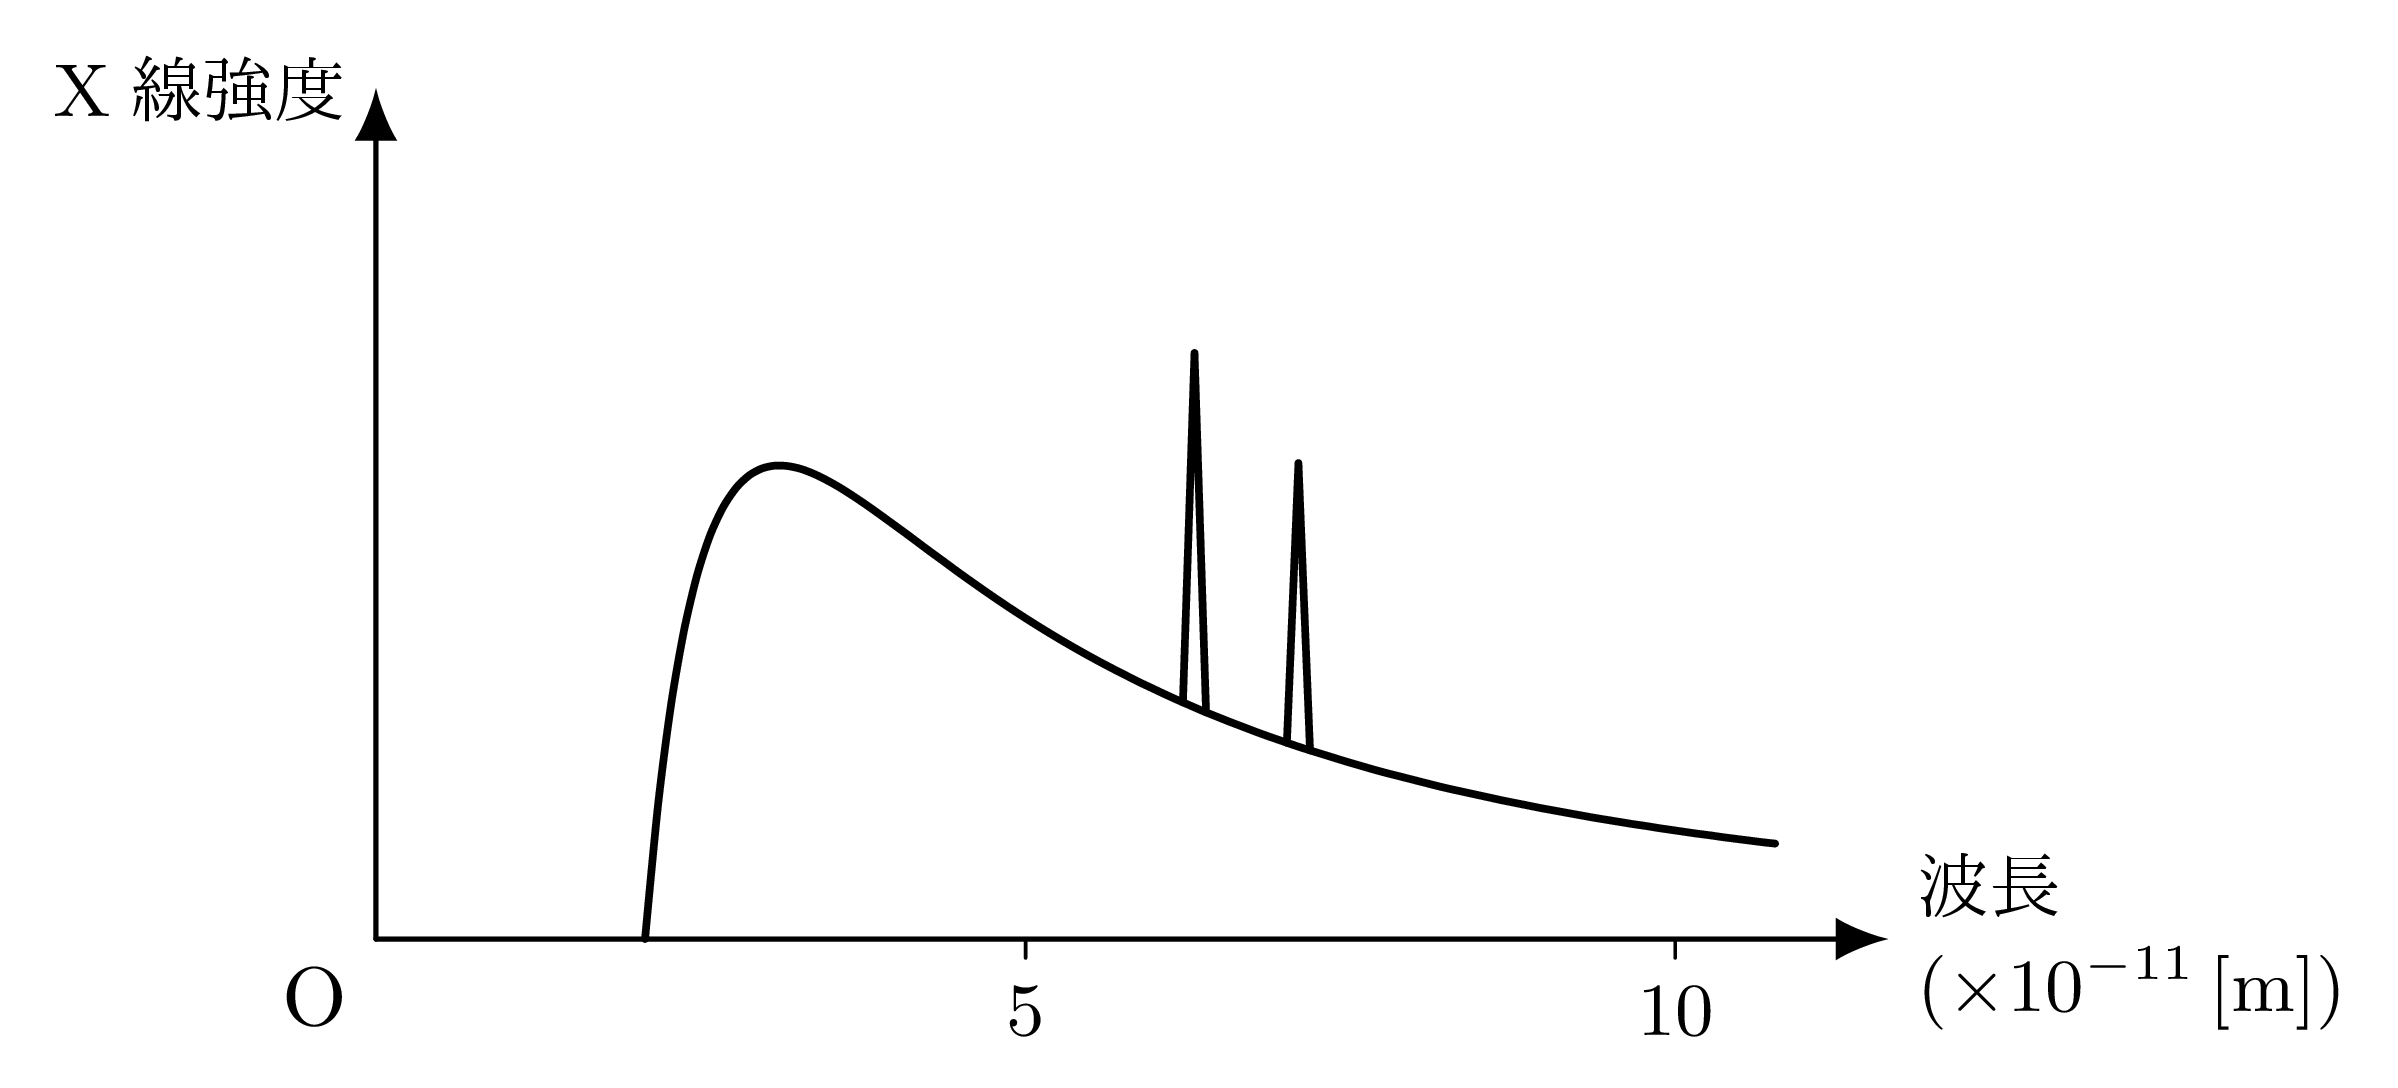
\includegraphics[keepaspectratio,width=60mm]{fig/n34_ex8_zu.png}
\end{zuright}
\end{reidai}

\begin{sisinE}
$eV$の大半が熱に，一部が$h\nu$になる．最短波長は加速電圧で決まり，特性X線の波長は加速電圧によらない．加速電圧を下げると電子1個のエネルギーが減るので，X線全体の強度も小さくなる．
\end{sisinE}

\Key{X線の最短波長は電圧によって決まる\quad 特性X線の波長は加速電圧によらない}

\begin{kaitou}
\begin{komon}
\ko{1} \[\lambda_{\min}=\frac{hc}{eV}=\frac{6.63\times 10^{-34}\times 3.00\times 10^8}{1.60\times 10^{-19}\times 60\times 10^3}\fallingdotseq 2.1\times 10^{-11}\U{m}\Ans\]
\ko{2} 加速電圧が半分になると最短波長は2倍の$4.1\times 10^{-11}\U{m}$になる．電子1個のエネルギーが減るので連続X線の強度は全体に小さくなるが，特性X線のピークの波長は変わらない．次図の破線のようになる．\Ans
       \begin{center}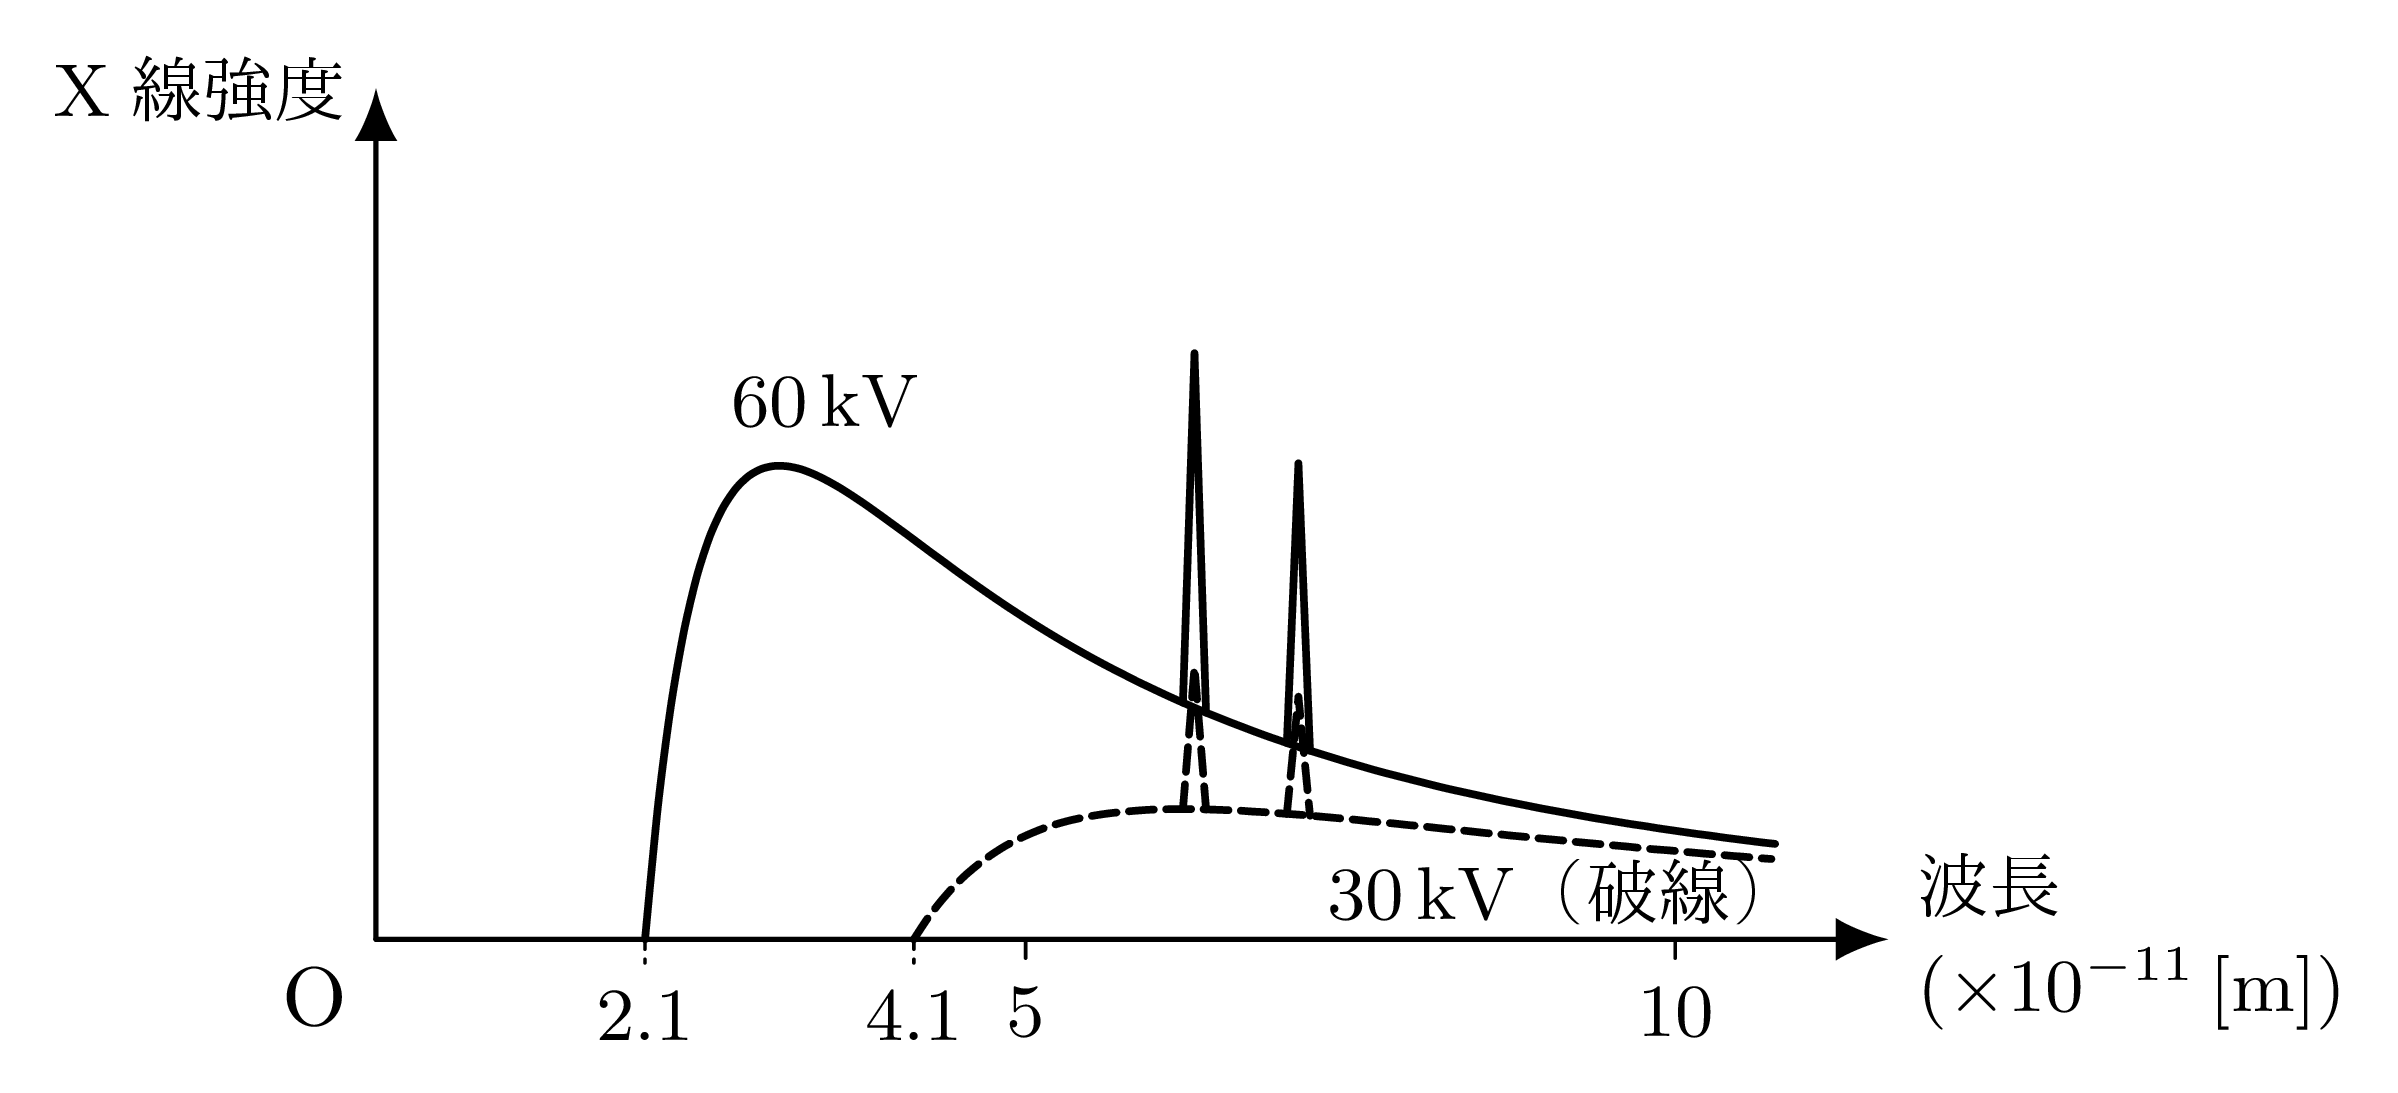
\includegraphics[keepaspectratio,width=62mm]{fig/n34_ex8_ans.png}\end{center}
\end{komon}
\end{kaitou}
\end{reidaiunit}

\subsection{ブラッグの条件}

\begin{zuright}{62mm}
\hspace{1zw}X線は電磁波であるから，光と同様に回折や干渉といった現象を起こす．
結晶の原子の間隔とほぼ同じ程度の波長のX線（例えば銅の特性X線の1つである$K_\alpha$線の波長は$0.154\U{nm}$程度）を用いて回折・干渉現象を利用すると，結晶の格子定数を精密に測定できる．

\hspace{1zw}図のように規則正しく配列した結晶を考える．平行な原子面の集合は\MARU{1}や\MARU{2}，\MARU{3}などさまざまなものが考えられるが，このうち\MARU{1}の原子面に着目し，この原子面に対して図のような角度$\theta$でX線を入射する．
隣り合う原子面で反射する2つのX線の経路差は，面間隔$d$を用いて$2d\sin\theta$であるので
\[2d\sin\theta=n\lambda\quad(n=1,2,3,\cdots)\]
の関係式が成立するような角度$\theta$でX線の強め合いが起こる．
この条件式を{\gtfamily ブラッグの条件}という．
逆に，強め合いの角度$\theta$を調べることにより，原子面の間隔を求めることができる．
\zusep

\includegraphics[keepaspectratio,width=60mm]{text2_p110_fig1.png}
\end{zuright}

% 加筆：電子線の回折（練習［12］［19］）．
第33回で学んだように電子も波（物質波）の性質を持つので，電子線を結晶に当てると，X線と同じくブラッグの条件を満たす角度で強め合う（デヴィッソン・ジャーマーの実験）．このとき$\lambda$には電子のド・ブロイ波長$\lambda=\dfrac{h}{mv}$を使えばよい．

\bsNeed{20mm}
\begin{matome}{ブラッグの条件}
 \hspace{3mm} \AnaB{$2d\sin\theta=n\lambda$}\quad（$n=1,2,3,\cdots$）\quad $\theta$は原子面と入射X線（電子線）のなす角
\end{matome}

\subsection{原子核の構成・同位体・原子質量単位}

\begin{zuright}{46mm}
\hspace{1zw}原子は原子核と電子から構成されているが，さらに細かく分解すると，原子核は$+e$の正電荷を持つ{\gtfamily 陽子}（プロトン，${}^1_1\mathrm{p}$）と電気的に中性な{\gtfamily 中性子}（ニュートロン，${}^1_0\mathrm{n}$）とが{\gtfamily 核力}と呼ばれる力で結合して作られている．陽子と中性子をまとめて{\gtfamily 核子}と呼ぶ．

\hspace{1zw}原子番号が$Z$の原子核は$Z$個の陽子を持つ．原子核が$N$個の中性子を持つ場合，陽子数と中性子数の和$A=Z+N$を{\gtfamily 質量数}と呼ぶ．
また，原子番号$Z$の元素記号を$\mathrm{X}$とすると，原子番号$Z$，質量数$A$の原子核を持つ原子を${}^A_Z\mathrm{X}$と表す．
すなわち電気的に中性な原子${}^A_Z\mathrm{X}$は，右図にあるように，$Z$個の陽子と$A-Z$個の中性子とからなる原子核のまわりを，$Z$個の電子が回っている．
\zusep

\includegraphics[keepaspectratio,width=44mm]{text2_p111_fig1.png}
\end{zuright}

陽子の数（原子番号$Z$）は等しいが，中性子の数$N=A-Z$が異なる原子のことを{\gtfamily 同位体}（アイソトープ）という．
同位体とは原子核の電荷は同じだが原子核の質量が異なるもの，とも言える．
一般に，化学反応は電荷（電子の配置）によってその反応が決まり，質量は大きな影響を及ぼさない．そのため，同位体同士では化学的性質の差はほとんどない．

また，原子1個の質量は極めて小さいので，$\mathrm{kg}$を単位とするのは面倒である．
そこで，炭素の同位体の1つである${}^{12}_{\ 6}\mathrm{C}$の質量を$12\U{u}$とし，これとの相対質量として質量をはかる．この単位を{\gtfamily 原子質量単位}という．
${}^{12}_{\ 6}\mathrm{C}$が$1\U{mol}$（$6.02\times 10^{23}$個）あるときの質量は$12\U{g}$であるから
\[1\U{u}=\frac{12\times 10^{-3}\U{kg}}{6.02\times 10^{23}}\times\frac{1}{12}\fallingdotseq 1.66\times 10^{-27}\U{kg}\]
と換算できる．陽子，中性子，電子の質量$m_{\mathrm{p}}$，$m_{\mathrm{n}}$，$m_{\mathrm{e}}$は，大まかに$m_{\mathrm{p}}\fallingdotseq m_{\mathrm{n}}\fallingdotseq 1\U{u}$，$m_{\mathrm{e}}\fallingdotseq\dfrac{1}{1800}\U{u}$であり，原子${}^A_Z\mathrm{X}$の質量はおよそ$A\U{u}$である．
元素の原子量は，各同位体の質量（$\U{u}$単位）に天然の同位体存在比をかけて足し合わせた平均値である．

\bsNeed{30mm}
\begin{matome}{原子核の構成・同位体・原子質量単位}
 \hspace{3mm} ${}^A_Z\mathrm{X}$は\AnaB{陽子$Z$個}，\AnaB{中性子$A-Z$個}を持つ\qquad 同位体：陽子数が等しく中性子数が異なる原子\\
 \hspace{3mm} $1\U{u}\fallingdotseq 1.66\times 10^{-27}\U{kg}$\qquad $m_{\mathrm{p}}\fallingdotseq m_{\mathrm{n}}\fallingdotseq 1\U{u}$，$m_{\mathrm{e}}\fallingdotseq\dfrac{1}{1800}\U{u}$
\end{matome}

%%%%%%%%%%  例題9（原本の【例題9】）  %%%%%%%%%%%%%%%%%%%%
\bsNeed{50mm}
\begin{reidaiunit}
\begin{reidai}{同位体}
\hspace{1zw}次の表に示されるような\MARU{1}〜\MARU{7}の中性原子がある．これについて，以下の設問に答えよ．なお，原子番号が88，89，90の元素はそれぞれ$\mathrm{Ra}$，$\mathrm{Ac}$，$\mathrm{Th}$である．
\begin{center}
\begin{tabular}{c|ccccccc}
原子 & \MARU{1} & \MARU{2} & \MARU{3} & \MARU{4} & \MARU{5} & \MARU{6} & \MARU{7}\\ \hline
質量数 & 224 & 226 & 228 & 228 & 228 & 232 & 234\\
核外電子数 & 88 & 88 & 88 & 89 & 90 & 90 & 90
\end{tabular}
\end{center}
\begin{komon}
\ko{1} 原子核を構成している中性子の数が同じ原子はどれとどれか．
\ko{2} 原子\MARU{1}と同位体の関係にある原子はどれか．
\ko{3} \MARU{1}〜\MARU{7}の原子を表す記号を書け．
\end{komon}
\end{reidai}

\begin{sisinE}
中性原子では核外電子数＝陽子数＝原子番号$Z$である．中性子数は$A-Z$．
\end{sisinE}

\Key{原子番号$Z$＝陽子数，質量数$A$\ $\Rightarrow$\ $A-Z$個の中性子を持つ}

\begin{kaitou}
中性子数$A-Z$はそれぞれ\MARU{1}136，\MARU{2}138，\MARU{3}140，\MARU{4}139，\MARU{5}138，\MARU{6}142，\MARU{7}144である．
\begin{komon}
\ko{1} \MARU{2}と\MARU{5}\Ans
\ko{2} 原子番号（陽子数）が88で等しい\MARU{2}，\MARU{3}\Ans
\ko{3} \MARU{1}${}^{224}_{\ 88}\mathrm{Ra}$\quad \MARU{2}${}^{226}_{\ 88}\mathrm{Ra}$\quad \MARU{3}${}^{228}_{\ 88}\mathrm{Ra}$\quad \MARU{4}${}^{228}_{\ 89}\mathrm{Ac}$\quad \MARU{5}${}^{228}_{\ 90}\mathrm{Th}$\quad \MARU{6}${}^{232}_{\ 90}\mathrm{Th}$\quad \MARU{7}${}^{234}_{\ 90}\mathrm{Th}$\Ans
\end{komon}
\end{kaitou}
\end{reidaiunit}

\subsection{放射壊変と変位法則}

原子において，電子に安定状態（基底状態）と不安定状態（励起状態）があったように，原子核にも安定な状態と不安定な状態とがある．
不安定な原子核は，{\gtfamily 放射線}と呼ばれるものを放出することで過剰なエネルギーを放出し，安定な状態へと変化していく．
この現象を{\gtfamily 放射壊変}（崩壊）といい，放射線を出す性質を{\gtfamily 放射能}，放射能を持つ物質を{\gtfamily 放射性物質}という．
放射線には$\alpha$線，$\beta$線，$\gamma$線の3種類があり，その正体と性質は次の通りである．

\bsNeed{26mm}
\begin{matome}{放射線の正体}
 \hspace{3mm} \MARU{1}\ $\alpha$線：\AnaB{ヘリウムの原子核${}^4_2\mathrm{He}$}の流れ\quad \MARU{2}\ $\beta$線：高速な\AnaB{電子}${}^{\ \ 0}_{-1}\mathrm{e}$の流れ\quad \MARU{3}\ $\gamma$線：波長の極めて短い\AnaB{電磁波}（光子）
\end{matome}

\begin{center}

\includegraphics[keepaspectratio,width=150mm]{text2_p113_fig1.png}
\end{center}

$\alpha$線，$\beta$線，$\gamma$線を出す放射壊変を，それぞれ$\alpha$崩壊，$\beta$崩壊，$\gamma$崩壊という．

\begin{zuright}{34mm}
\noindent\MARU{1}\ {\gtfamily $\alpha$崩壊}\par
\hspace{1zw}${}^{238}_{\ 92}\mathrm{U}$や${}^{232}_{\ 90}\mathrm{Th}$などは，質量数$A$が大きすぎるため，表面付近にいる陽子や中性子の結合が弱い．そのため，陽子2個，中性子2個がひとかたまり（${}^4_2\mathrm{He}$原子核）となって外れる．この結果，{\gtfamily 陽子数は2減少（$\Delta Z=-2$），質量数は4減少（$\Delta A=-4$）}する．反応式で${}^A_Z\mathrm{X}\to{}^{A^\prime}_{Z^\prime}\mathrm{Y}+{}^4_2\mathrm{He}$となるとき，$A=A^\prime+4$，$Z=Z^\prime+2$が成立する．
\zusep

\includegraphics[keepaspectratio,width=30mm]{text2_p114_fig1.png}
\end{zuright}

\begin{zuright}{34mm}
\noindent\MARU{2}\ {\gtfamily $\beta$崩壊}\par
\hspace{1zw}原子番号$Z$が小さい範囲では$N\fallingdotseq Z$ぐらいの中性子数が，$Z$が大きい範囲では$N\fallingdotseq 1.6Z$程度の中性子数のときに原子核は安定であるが，中性子数が多すぎるときには原子核中の中性子が電子を放出して陽子に変化する．この結果，{\gtfamily 陽子数は1増加（$\Delta Z=+1$），質量数は不変（$\Delta A=0$）}である．反応式で${}^A_Z\mathrm{X}\to{}^{A^\prime}_{Z^\prime}\mathrm{Y}+{}^{\ \ 0}_{-1}\mathrm{e}$となるとき，$A=A^\prime$，$Z=Z^\prime-1$が成立する（電子を質量数0，陽子数$-1$の粒子とみなせば，$\alpha$崩壊と同様に全質量数と全陽子数が保存している）．
\zusep

\includegraphics[keepaspectratio,width=30mm]{text2_p114_fig2.png}
\end{zuright}

\begin{zuright}{34mm}
\noindent\MARU{3}\ {\gtfamily $\gamma$崩壊}\par
\hspace{1zw}$\alpha$崩壊，$\beta$崩壊した直後の原子核は高いエネルギーを持った不安定な状態（励起状態）にある．これが安定な状態になるとき，その差のエネルギーが光子として放出される．このとき{\gtfamily 荷電粒子の放出はなく，光子（電磁波）が放出される}ので，陽子数，質量数はいずれも不変である．
\zusep

\includegraphics[keepaspectratio,width=30mm]{text2_p114_fig3.png}
\end{zuright}

\bsNeed{26mm}
\begin{matome}{放射壊変}
 \hspace{3mm} 反応式を書いて，崩壊の前後で\AnaB{全質量数}（左上の数の和）と\AnaB{全陽子数}（左下の数の和）の保存を考える\\
 \hspace{3mm} （電子は質量数0，陽子数$-1$の粒子${}^{\ \ 0}_{-1}\mathrm{e}$とみなす）
\end{matome}

%%%%%%%%%%  例題10（原本の【例題10】）  %%%%%%%%%%%%%%%%%%%%
\bsNeed{50mm}
\begin{reidaiunit}
\begin{reidai}{放射壊変}
\hspace{1zw}${}^{238}_{\ 92}\mathrm{U}$が自然放射を繰り返して最終的に${}^{206}_{\ 82}\mathrm{Pb}$になった．これについて以下の設問に答えよ．
\begin{komon}
\ko{1} この放射壊変における$\alpha$崩壊を$x$回，$\beta$崩壊を$y$回とする．このとき，この放射壊変の反応式を示せ．
\ko{2} 全質量数保存の式および全陽子数保存の式を示せ．
\ko{3} ${}^{238}_{\ 92}\mathrm{U}$から${}^{206}_{\ 82}\mathrm{Pb}$になるまでの$\alpha$崩壊，$\beta$崩壊の回数をそれぞれ求めよ．
\end{komon}
\end{reidai}

\begin{sisinE}
$\alpha$崩壊では${}^4_2\mathrm{He}$，$\beta$崩壊では${}^{\ \ 0}_{-1}\mathrm{e}$が放出される．これらを$x$個，$y$個並べた反応式を書き，左上・左下の数の和をそろえる．
\end{sisinE}

\Key{放射壊変\ $\Rightarrow$\ 必ず反応式を考えて，全質量数・全陽子数保存の式を立てる}

\begin{kaitou}
\begin{komon}
\ko{1} \[{}^{238}_{\ 92}\mathrm{U}\to{}^{206}_{\ 82}\mathrm{Pb}+x\,{}^4_2\mathrm{He}+y\,{}^{\ \ 0}_{-1}\mathrm{e}\Ans\]
\ko{2} \[\text{質量数：}\ 238=206+4x,\qquad\text{陽子数：}\ 92=82+2x-y\Ans\]
\ko{3} (2)を解いて$x=8$，$y=6$．\quad $\alpha$崩壊8回，$\beta$崩壊6回\Ans
\end{komon}
\end{kaitou}
\end{reidaiunit}

\subsection{自然放射系列と半減期}

原子番号が83以上の元素には不安定な同位体が多く，これらは自然に（外部からの刺激なしに）放射線を出して壊変していく．
質量数$A$の変化は，$\alpha$崩壊では$-4$だが，$\beta$崩壊，$\gamma$崩壊では変化しないため，{\gtfamily 放射壊変では質量数は4ずつしか変化できない}．
そのため，天然に存在する放射性元素は，質量数$A$を4で割った余りによって，ウラン系列（$A=4n+2$，${}^{238}_{\ 92}\mathrm{U}\to{}^{206}_{\ 82}\mathrm{Pb}$），アクチニウム系列（$A=4n+3$，${}^{235}_{\ 92}\mathrm{U}\to{}^{207}_{\ 82}\mathrm{Pb}$），トリウム系列（$A=4n$，${}^{232}_{\ 90}\mathrm{Th}\to{}^{208}_{\ 82}\mathrm{Pb}$），ネプツニウム系列（$A=4n+1$，${}^{237}_{\ 93}\mathrm{Np}\to{}^{209}_{\ 83}\mathrm{Bi}$）の4通りに分類される．
% 原本（physics_ch46.tex）はネプツニウム系列の終点を「${}^{209}_{82}$Pb」としていたが，${}^{209}_{\ 83}$Bi（ビスマス）が正しい．

\begin{zuright}{50mm}
\hspace{1zw}放射性元素が崩壊していく速さは，核種（崩壊する原子核の種類）によって決まり，圧力や温度などの外部条件によらない．
ある同種の原子核が$N$個あるとすると，原子核が崩壊する確率はどの核についても等しいから，微小時間$\Delta t$の間に崩壊する原子核の個数は$\Delta t$と$N$に比例する．比例定数を$\lambda$として$\Delta N=-\lambda N\Delta t$が成立し，これを解くと，時刻$t=0$に原子核が$N_0$個あったとして$N=N_0e^{-\lambda t}$となる．
これより原子核の個数は指数関数的に減少していく．

\hspace{1zw}もともとあった原子核数がちょうど半分になるまでの時間$T$を{\gtfamily 半減期}と呼ぶ．$T$を用いると
\[\frac{N}{N_0}=\Bigl(\frac{1}{2}\Bigr)^{\frac{t}{T}}\]
となる．時刻$t$が$T$だけ増すとちょうど$\dfrac{1}{2}$がかかった形になるので，半減期とは，{\gtfamily 現在存在する量がちょうど半分になるのに要する時間}である．半減期が短い原子核ほど不安定である．
\zusep

\includegraphics[keepaspectratio,width=48mm]{text2_p116_fig1.png}
\end{zuright}

\bsNeed{22mm}
\begin{matome}{半減期}
 \hspace{3mm} 半減期$T$＝現在存在する量がちょうど半分になるのに要する時間\qquad \AnaB{$\dfrac{N}{N_0}=\Bigl(\dfrac{1}{2}\Bigr)^{\frac{t}{T}}$}
\end{matome}

%%%%%%%%%%  例題11（原本の【例題11】）  %%%%%%%%%%%%%%%%%%%%
\bsNeed{44mm}
\begin{reidaiunit}
\begin{reidai}{半減期}
\hspace{1zw}${}^{226}_{\ 88}\mathrm{Ra}$は半減期1622年で自然崩壊して${}^{222}_{\ 86}\mathrm{Rn}$に変化する．これについて以下の設問に答えよ．
\begin{komon}
\ko{1} ${}^{226}_{\ 88}\mathrm{Ra}$の量が現在の$\dfrac{1}{16}$の量になるのは何年後か．
\ko{2} 3244年前には，現在の量の何倍あったか．
\end{komon}
\end{reidai}

\begin{sisinE}
(1) $\dfrac{1}{16}$になるためには，半分になるのを何回繰り返せばよいかを考える．
(2) 3244年間というのは半減期の何倍かを考える．
\end{sisinE}

\Key{半減期$T$＝現在存在する量がちょうど半分になるのに要する時間}

\begin{kaitou}
\begin{komon}
\ko{1} $\dfrac{1}{16}=\Bigl(\dfrac{1}{2}\Bigr)^4$より，半分になるのを4回繰り返せばよいので\quad $1622\times 4=6488$年後\Ans
\ko{2} $3244=1622\times 2$年前には，半分になる前の量をさらに2回さかのぼるので\quad $2^2=4$倍\Ans
\end{komon}
\end{kaitou}
\end{reidaiunit}

\subsection{原子核反応}

原子核に$\alpha$粒子（${}^4_2\mathrm{He}$）や陽子（${}^1_1\mathrm{p}$），中性子（${}^1_0\mathrm{n}$）などをぶつけると，その原子核が他の原子核に変化することがある．この反応を{\gtfamily 原子核反応}という．原子核反応の前後では，次の4つの量が保存される．

\bsNeed{24mm}
\begin{matome}{原子核反応}
 \hspace{3mm} \MARU{1}\ 全陽子数（反応式の左下の数の和）\quad \MARU{2}\ 全質量数（左上の数の和）\quad \MARU{3}\ 全運動量\quad \MARU{4}\ 質量エネルギーを含めた全エネルギー
\end{matome}

ここではまず\MARU{1}\MARU{2}について考える．通常，原子核反応では電子を持たない原子核同士を反応させるため，各粒子は正に帯電しているが，右上の電荷は書かずに省略するのが通例である．
陽子や中性子，電子は${}^1_1\mathrm{p}$，${}^1_0\mathrm{n}$，${}^{\ \ 0}_{-1}\mathrm{e}$というように質量数，陽子数をつけて考えるとよい．
また，水素（陽子数1）には中性子数が0，1，2の3つの同位体があり，それぞれ水素，重水素，三重水素と呼ばれる．重水素，三重水素はそれぞれ$\mathrm{D}$，$\mathrm{T}$と書かれることが多い．水素原子核${}^1_1\mathrm{H}$は陽子${}^1_1\mathrm{p}$そのものである．
\[{}^1_1\mathrm{H}={}^1_1\mathrm{p},\qquad{}^2_1\mathrm{H}={}^2_1\mathrm{D},\qquad{}^3_1\mathrm{H}={}^3_1\mathrm{T}\]

%%%%%%%%%%  例題12（原本の【例題12】）  %%%%%%%%%%%%%%%%%%%%
\bsNeed{40mm}
\begin{reidaiunit}
\begin{reidai}{原子核反応}
\hspace{1zw}次の原子核反応式の（\hspace{2zw}）に適当なものを記入して反応式を完成させよ．
\begin{komon}
\ko{1} ${}^9_4\mathrm{Be}+{}^4_2\mathrm{He}\to(\hspace{3zw})+{}^1_0\mathrm{n}$
\ko{2} ${}^{12}_{\ 6}\mathrm{C}+{}^2_1\mathrm{H}\to(\hspace{3zw})+{}^1_1\mathrm{H}$
\end{komon}
\end{reidai}

\begin{sisinE}
反応式の左上（質量数）と左下（陽子数）の数の和が反応の前後で等しくなるようにする．陽子数から元素が決まる．
\end{sisinE}

\Key{原子核反応では，\MARU{1}全陽子数\ \MARU{2}全質量数\ \MARU{3}全運動量\ \MARU{4}全エネルギーが保存}

\begin{kaitou}
\begin{komon}
\ko{1} 陽子数$4+2-0=6$，質量数$9+4-1=12$より\quad ${}^{12}_{\ 6}\mathrm{C}$\Ans
\ko{2} 陽子数$6+1-1=6$，質量数$12+2-1=13$より\quad ${}^{13}_{\ 6}\mathrm{C}$\Ans
\end{komon}
\end{kaitou}
\end{reidaiunit}

\subsection{質量とエネルギーの等価性}

アインシュタインは1905年に，相対性理論の中で，{\gtfamily 質量とエネルギーは同等で，相互に変換しうるものである}ことを示した．
この理論によれば，質量$m$はエネルギー
\AnaBD{E=mc^2}
に相当し，これを{\gtfamily 質量エネルギー}という．この関係式を用いると，原子核反応の際に発生するエネルギーや，原子核の結合エネルギーを計算することができる．

\begin{zuright}{62mm}
\hspace{1zw}陽子，中性子の質量を$m_{\mathrm{p}}$，$m_{\mathrm{n}}$とする．陽子$Z$個，中性子$N$個から形成される原子核の質量$M$は，核を構成している陽子，中性子をばらばらにして足し合わせた質量の和$Zm_{\mathrm{p}}+Nm_{\mathrm{n}}$よりも小さくなる．この差
\[\Delta m=Zm_{\mathrm{p}}+Nm_{\mathrm{n}}-M\]
を{\gtfamily 質量欠損}と呼ぶ．
エネルギー図で表すと右図のようになり，核子が結合することによって，この差のエネルギー分だけ安定化したことになる．逆に言えば，原子核をばらばらにするのにこの差のエネルギーが必要であるから，この差は原子核の{\gtfamily 結合エネルギー}を表している．
\[\Delta E=(Zm_{\mathrm{p}}+Nm_{\mathrm{n}})c^2-Mc^2=\Delta m\cdot c^2\]
\zusep

\includegraphics[keepaspectratio,width=60mm]{text2_p119_fig1.png}
\end{zuright}

\begin{zuright}{62mm}
\hspace{1zw}核子1個あたりの結合エネルギー$\dfrac{\Delta E}{A}$を{\gtfamily 比結合エネルギー}という．各原子核の比結合エネルギーをグラフにしたものを右図に示す．
グラフから分かるように，原子核は$\mathrm{Fe}$付近が最も安定である．そのため，{\gtfamily 質量数の大きい原子核は分裂することにより安定化しようとする}．これが{\gtfamily 核分裂}であり，原子力発電所では，原子炉で核分裂を連鎖的に起こし，そのときに発生するエネルギーを利用して発電している．一方，{\gtfamily 質量数の小さい原子核は結合することにより安定化しようとする}．これが{\gtfamily 核融合}であり，太陽などの恒星では核融合で発生したエネルギーが光や熱として放出されている．
\zusep

\includegraphics[keepaspectratio,width=60mm]{text2_p119_fig2.png}
\end{zuright}

核分裂による発電では，半減期が長い放射性物質が生じてしまうため，放射性廃棄物をどう処理するかが問題となる．一方で，核融合で生じる物質は半減期が短く，燃料となる水素などの資源も豊富であるため，将来のエネルギー源の1つとして期待されている．しかし，互いに正の電荷を持った原子核同士を衝突させるには，クーロン力に打ち勝つだけの運動エネルギーが必要となり（練習［21］），超高温（かつ高密度）に保つ必要がある．

% 加筆：原子核反応で発生するエネルギー（練習［20］）．
原子核反応でも同様に，{\gtfamily 反応前の質量の和と反応後の質量の和の差$\Delta M$に相当するエネルギー$\Delta Mc^2$が放出される}（反応後の方が軽いとき）．このエネルギーは生成した粒子の運動エネルギーや$\gamma$線のエネルギーになる．
原子核の質量は$\U{u}$単位で与えられることが多いので，$1\U{u}$の質量エネルギーを覚えておくと便利である（例題13）．

%%%%%%%%%%  例題13（原本の【例題13】）  %%%%%%%%%%%%%%%%%%%%
\bsNeed{50mm}
\begin{reidaiunit}
\begin{reidai}{質量欠損}
\hspace{1zw}以下の設問に答えよ．ただし，$1\U{u}=1.66\times 10^{-27}\U{kg}$，光速$c=3.00\times 10^8\U{m/s}$，電気素量$e=1.60\times 10^{-19}\U{C}$，陽子の質量は$m_{\mathrm{p}}=1.0073\U{u}$，中性子の質量は$m_{\mathrm{n}}=1.0087\U{u}$である．
\begin{komon}
\ko{1} $1\U{u}$と等価なエネルギーを，$\U{MeV}$（メガエレクトロンボルト）単位で表せ．
\ko{2} ヘリウム原子核の質量は$4.0015\U{u}$である．ヘリウム原子核の結合エネルギーを求めよ．
\end{komon}
\end{reidai}

\begin{sisinE}
(1) $E=mc^2$で計算し，$1\U{MeV}=10^6\U{eV}=1.60\times 10^{-13}\U{J}$で換算する．
(2) 原子核の結合エネルギーは，ばらばらにしたときとの質量の差（質量欠損）のエネルギーである．
\end{sisinE}

\Key{質量エネルギー$E=mc^2$\quad 結合エネルギー＝ばらばらのときとの質量エネルギーの差}

\begin{kaitou}
\begin{komon}
\ko{1} \[E=1.66\times 10^{-27}\times(3.00\times 10^8)^2\fallingdotseq 1.494\times 10^{-10}\U{J}\]
       \[\frac{1.494\times 10^{-10}}{1.60\times 10^{-13}}\U{MeV}\fallingdotseq 9.34\times 10^2\U{MeV}\Ans\]
       （より精密な定数を用いると$931.5\U{MeV}$となる．）
\ko{2} ヘリウム原子核${}^4_2\mathrm{He}$は陽子2個，中性子2個からなるので，質量欠損は
       \[\Delta m=2\times 1.0073+2\times 1.0087-4.0015=0.0305\U{u}\]
       よって結合エネルギーは\quad $0.0305\times 9.34\times 10^2\fallingdotseq 28.5\U{MeV}$\Ans
\end{komon}
\end{kaitou}
\end{reidaiunit}

\bsNeed{18mm}
\begin{matome}{質量とエネルギーの関係}
 \hspace{3mm} $1\U{u}$の質量は約\AnaB{$931\U{MeV}$}のエネルギーに相当する\qquad 結合エネルギー$\Delta E=\Delta m\cdot c^2$
\end{matome}

%%%%%%%%%%  例題14（原本の【例題14】）  %%%%%%%%%%%%%%%%%%%%
\bsNeed{56mm}
\begin{reidaiunit}
\begin{reidai}{核融合反応}
\hspace{1zw}2個の重陽子（重水素の原子核）が次のような原子核反応を起こした．
\[{}^2_1\mathrm{H}+{}^2_1\mathrm{H}\to{}^3_2\mathrm{He}+{}^1_0\mathrm{n}\]
これについて以下の設問に答えよ．ただし，各粒子の質量は${}^2_1\mathrm{H}$：$2.0136\U{u}$，${}^3_2\mathrm{He}$：$3.0149\U{u}$，${}^1_0\mathrm{n}$：$1.0087\U{u}$である．また，$1\U{u}$は$931\U{MeV}$に相当することを用いてよい．
\begin{komon}
\ko{1} この原子核反応で発生するエネルギーを，$\U{MeV}$単位で求めよ．
\ko{2} 2個の重陽子が互いに等しい運動エネルギー$0.35\U{MeV}$で正面衝突した．このとき，原子核反応で発生した中性子とヘリウム原子核はそれぞれどれだけの運動エネルギーを持つか．$\U{MeV}$単位で答えよ．
\end{komon}
\end{reidai}

\begin{sisinE}
(1) 反応前後の質量の差に相当するエネルギーが発生する．
(2) 正面衝突なので衝突前の全運動量は$0$．反応後の2粒子は逆向きに同じ大きさの運動量で飛び出す．運動量の大きさが等しいとき，運動エネルギー$\dfrac{p^2}{2m}$は質量に反比例する（質量は質量数で近似してよい）．
\end{sisinE}

\Key{原子核反応では，\MARU{1}全陽子数\ \MARU{2}全質量数\ \MARU{3}全運動量\ \MARU{4}全エネルギーが保存}

\begin{kaitou}
\begin{komon}
\ko{1} 質量の減少は$2\times 2.0136-(3.0149+1.0087)=0.0036\U{u}$であるから
       \[\Delta E=0.0036\times 931\fallingdotseq 3.4\U{MeV}\Ans\]
\ko{2} エネルギー保存則より，反応後の運動エネルギーの和は$K_{\mathrm{n}}+K_{\mathrm{He}}=0.35\times 2+3.35=4.05\U{MeV}$．
       運動量保存則より中性子とヘリウム原子核の運動量の大きさ$p$は等しいので，$K=\dfrac{p^2}{2m}$より$K_{\mathrm{n}}:K_{\mathrm{He}}=m_{\mathrm{He}}:m_{\mathrm{n}}\fallingdotseq 3:1$．よって
       \[K_{\mathrm{n}}=4.05\times\frac{3}{4}\fallingdotseq 3.0\U{MeV},\qquad K_{\mathrm{He}}=4.05\times\frac{1}{4}\fallingdotseq 1.0\U{MeV}\Ans\]
\end{komon}
\end{kaitou}
\end{reidaiunit}

\subsection{素粒子}

原子核は陽子，中性子によって構成されているが，陽子，中性子は複数の{\gtfamily クォーク}の組み合わせからなることが分かった．
このように，物質を構成する要素とその相互作用について調べていくのが素粒子論であり，その理論を{\gtfamily 標準理論}と呼ぶ．
標準理論に基づく素粒子は，物質を構成する{\gtfamily フェルミ粒子}（物質粒子），力を伝達する{\gtfamily ゲージ粒子}，質量を与える{\gtfamily ヒッグス粒子}に分類される．
フェルミ粒子は，強い相互作用をする{\gtfamily クォーク}と強い相互作用をしない{\gtfamily レプトン}に分けられ，それぞれ6種類ずつあることが分かっている．これらは性質の似ている組に分けられ，次の表のように第1世代，第2世代，第3世代に分けられている．
\begin{center}

\includegraphics[keepaspectratio,width=140mm]{text2_p121_fig1.png}
\end{center}

これらのクォーク，レプトンには，対応する{\gtfamily 反粒子}が存在する．例えば，電子の反粒子は{\gtfamily 陽電子}（ポジトロン）と呼ばれ，質量は電子と同じであるが，$+e$に帯電している（反応式では${}^0_1\mathrm{e}^+$と書く．練習［16］(4)）．
粒子と反粒子が衝突すると{\gtfamily 対消滅}し，その際に失われた質量エネルギーは光子などに変換される．逆に，光子などのエネルギーから粒子と反粒子が{\gtfamily 対生成}することもある．

陽子，中性子は3つのクォークから形成されていて，
\[\text{陽子：アップ2つ＋ダウン1つ}\ \Bigl(\frac{2}{3}e\times 2-\frac{1}{3}e=e\Bigr),\qquad\text{中性子：アップ1つ＋ダウン2つ}\ \Bigl(\frac{2}{3}e-\frac{1}{3}e\times 2=0\Bigr)\]
となる．クォークからなる粒子を{\gtfamily ハドロン}と呼び，陽子や中性子のように3つのクォークからなるハドロンを{\gtfamily バリオン}（重粒子），クォーク1つと反クォーク1つからなるハドロンを{\gtfamily メソン}（中間子）という（例えば$\pi^+$中間子はアップクォークと反ダウンクォークからなる）．中間子が核子間で交換されることにより，核力が生じる．

標準理論において，自然界に存在する力は4つに分類され，それぞれゲージ粒子によってその力が伝わり，相互作用していると考えられている．4つの力と，それに対応するゲージ粒子は次の表のようになる．ウィークボソンはヒッグス粒子により，質量を獲得したと考えられている．
\begin{center}

\includegraphics[keepaspectratio,width=140mm]{text2_p121_fig2.png}
\end{center}


\newpage

%%%%%%%%%%%%%%%%%%%%  練習問題  %%%%%%%%%%%%%%%%%%%%
% 第33回の［9］に続く．
\setcounter{qno}{9}

\filbreak
\Rank{A問題}

\Mon{基本事項の確認}

\hspace{1zw}以下の設問に答えよ．アボガドロ定数$N_{\mathrm{A}}=6.02\times 10^{23}\U{/mol}$，光速$c=3.0\times 10^8\U{m/s}$，電気素量は$e=1.6\times 10^{-19}\U{C}$である．
\begin{komon}
\ko{1} 次の文中の\BOX{ア}〜\BOX{キ}に適当な語句を埋めよ．\par
       ラザフォードの$\alpha$粒子の散乱実験から，原子の中心部には\BOX{ア}があることがわかった．\BOX{ア}の周りには$-e\U{C}$の電荷をもつ\BOX{イ}があり，\BOX{ア}は$+e\U{C}$の電荷をもつ\BOX{ウ}と電気的に中性な\BOX{エ}とから成っている．\BOX{ウ}と\BOX{エ}の数は原子の種類によって異なり，\BOX{ウ}の数は\BOX{オ}を表し，\BOX{ウ}の数と\BOX{エ}の数の和を\BOX{カ}という．\BOX{オ}が互いに等しい原子でも\BOX{カ}の異なる原子が存在し，それを\BOX{キ}という．
\ko{2} 塩素には質量数が35のものと37のものとがあり，原子量は約35.5である．質量数35の塩素原子は全体の何\%か．
\ko{3} 原子核反応では，中性子，電子の原子番号をそれぞれいくつとして扱うか．
\ko{4} 質量$1.0\times 10^3\U{kg}$に相当する質量エネルギーは何$\U{J}$か．
\ko{5} 半減期が1時間という放射性物質があるとする．3時間後には現在の何倍の量になるか．また現在の量の$\dfrac{1}{1024}$倍になるのは何時間後か．
\ko{6} 陽子のおおよその質量は何$\U{kg}$か．また，これは何$\U{MeV}$のエネルギーに相当するか．
\end{komon}

\filbreak
\Rank{B問題}

\Mon{X線の発生機構}

\hspace{1zw}以下の空欄\BOX{1}〜\BOX{5}に適当な語句または式を埋めよ．
\par
\hspace{1zw}高速の電子をタングステンのような原子量の大きい物質に当てると，X線が発生する．このとき発生するX線のスペクトルには，いろいろな波長が混じっている\BOX{1}X線と呼ばれる部分と，ある波長のところだけが急に強くなっている\BOX{2}X線と呼ばれる部分とがある．
\par
\hspace{1zw}電子がタングステンに当たって急に止まるとき，入射電子の持っている\BOX{3}がタングステンの熱エネルギーと光子（X線）のエネルギーとに転化される．このような機構で放出されるX線が\BOX{1}X線である．ここでプランク定数，光速をそれぞれ$h\U{J\cdot s}$，$c\U{m/s}$とし，また電子の電荷および加速電圧をそれぞれ$-e\U{C}$，$V\U{V}$とすれば，このような機構で発生するX線の最短波長$\lambda_{\min}\U{m}$は，電子の\BOX{3}がすべてX線のエネルギーになるような極限の場合であるから，$\lambda_{\min}=$\BOX{4}$\U{m}$となる．
\par
\hspace{1zw}また電子が原子に衝突してその内側の電子をたたき出すと，外側の軌道の電子がその軌道に落ち込んできて，そのときX線が放出される．このような機構で放出されるX線が\BOX{2}X線である．電子が外側の軌道を回っているときの全エネルギーを$E_1\U{J}$，内側の軌道を回っているときの全エネルギーを$E_2\U{J}$とすると，このような機構で発生するX線の波長は$\lambda_0=$\BOX{5}$\U{m}$となる．

\Mon[\Sitei]{ブラッグ反射条件・物質波}

\begin{zuright}{62mm}
\hspace{1zw}右図のように原子が整然と配列している結晶がある．今，電圧$V\U{V}$で加速された電子線が，この結晶の原子配列面$\mathrm{A}$，$\mathrm{B}$，$\mathrm{C}\cdots$に入射角$\theta$で入射し，各面で反射したとする．このとき電圧$V$を次第に増大させていくと，それに応じて入射電子線に対する反射電子線の強度の割合$R$には，極大極小が交互に現れる．プランク定数，電子の質量，電子の電荷をそれぞれ$h\U{J\cdot s}$，$m_{\mathrm{e}}\U{kg}$，$-e\U{C}$として以下の設問に答えよ．
\zusep
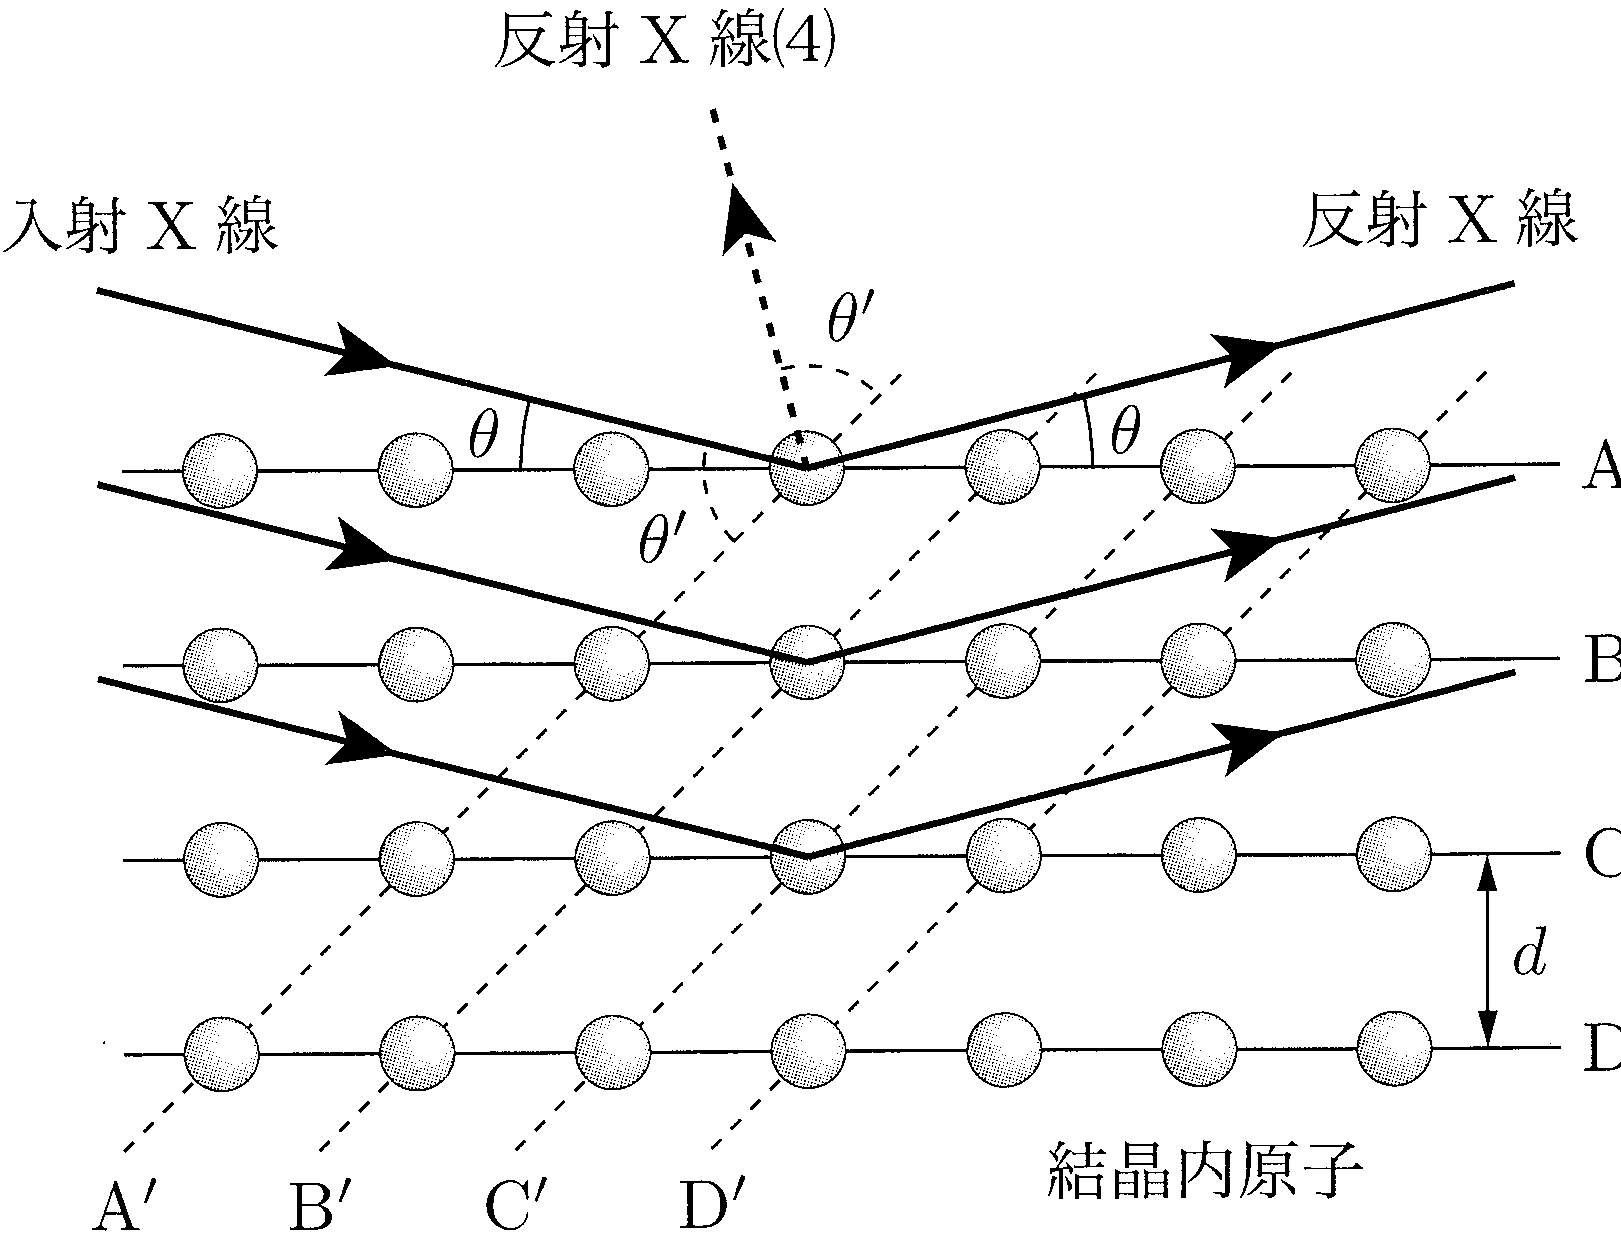
\includegraphics[keepaspectratio,width=60mm]{fig/n34_p12_zu.png}
\end{zuright}
\begin{komon}
\ko{1} 加速電圧が$V$のときの入射電子線の波長$\lambda\U{m}$を求めよ．
\ko{2} 強度の割合$R$が極大を示すとき，$d$，$\lambda$，$\theta$の間に成り立つ関係式を自然数$n$を用いて示せ．
\ko{3} 強度の割合$R$が極大を示すときの入射電子の加速電圧$V$を$n$を用いて示せ．
\ko{4} 図に波線で示した原子面$\mathrm{A^\prime}$，$\mathrm{B^\prime}$，$\mathrm{C^\prime}\cdots$（原子面$\mathrm{A}$，$\mathrm{B}$，$\mathrm{C}\cdots$に対して$45^\circ$だけ傾斜している）で散乱されてくる反射電子線が強め合うための条件を，電子線の波長$\lambda$，この原子面に対する電子線の入射する角度$\theta^\prime\ (=\theta+45^\circ)$，自然数$n$を用いて表せ．
\end{komon}

\Mon[\Sitei]{放射壊変}

\hspace{1zw}以下の空欄\BOX{1}〜\BOX{10}に適当な語句および式を埋めよ．ただし，変化については符号で増減を表せ．
\par
\hspace{1zw}原子核の$\alpha$崩壊によって放出される粒子の正体は\BOX{1}{\small（名称および原子を表す式を${}^A_Z\mathrm{X}^{n+}$の形で示せ）}であり，生じた新しい原子はもとの原子より原子番号は\BOX{2}だけ減少し，また質量数は\BOX{3}だけ減少する．それに対して原子核の$\beta$崩壊によって放出される粒子の正体は\BOX{4}{\small（1同様に示せ）}である．$\beta$崩壊の場合，原子番号は\BOX{5}だけ増加し，質量数は変わらない．また$\gamma$線は\BOX{6}であるが，特性X線の発生機構が原子の\BOX{7}に関係するのに対し，$\gamma$線は原子の\BOX{8}の状態変化によって放出される．これらの崩壊によって生じる放射線のうち電離作用が最も強いのは\BOX{9}であり，また透過力がもっとも強いのは\BOX{10}である．

\Mon{放射壊変の回数}

\hspace{1zw}ラジウム${}^{226}_{\ 88}\mathrm{Ra}$は$\alpha$崩壊と$\beta$崩壊とをそれぞれ何回か行って，鉛（原子番号82）の同位体になって安定する．以下の設問に答えよ．
\begin{komon}
\ko{1} 鉛の同位体の質量数を次の四つの値の中から選べ．\quad $204$，$205$，$206$，$207$
\ko{2} ラジウム${}^{226}_{\ 88}\mathrm{Ra}$が鉛になるまでに行った$\alpha$崩壊および$\beta$崩壊の回数を求めよ．
\end{komon}

\Mon{半減期}

\hspace{1zw}$\alpha$崩壊をする原子からできている物質がある．この物質は自然崩壊し，$12\U{s}$間で初めの量の$\dfrac{7}{8}$が他の物質に変化する．$\log_{10}2=0.3010$，$\log_{10}3=0.4771$として以下の設問に答えよ．
\begin{komon}
\ko{1} この物質の半減期$T\U{s}$を求めよ．
\ko{2} 現在の量の$\dfrac{2}{3}$になるまでの時間を求めよ．
\end{komon}

\Mon{原子核反応式}

\hspace{1zw}次の原子核反応式の空欄\framebox[4zw]{\rule{0pt}{1.1zw}}を正しく埋めて，完成せよ．
% 原本の(3)は「Ti」（チタン）だが，原子番号81はタリウム Tl．
\begin{komon}
\ko{1} ${}^9_4\mathrm{Be}+{}^4_2\mathrm{He}\to{}^{12}_{\ 6}\mathrm{C}+$\framebox[4zw]{\rule{0pt}{1.1zw}}
\ko{2} ${}^{14}_{\ 7}\mathrm{N}+{}^4_2\mathrm{He}\to{}^{17}_{\ 8}\mathrm{O}+$\framebox[4zw]{\rule{0pt}{1.1zw}}
\ko{3} ${}^{206}_{\ 81}\mathrm{Tl}\to{}^{206}_{\ 82}\mathrm{Pb}+$\framebox[4zw]{\rule{0pt}{1.1zw}}
\ko{4} ${}^{30}_{15}\mathrm{P}\to{}^{30}_{14}\mathrm{Si}+$\framebox[4zw]{\rule{0pt}{1.1zw}}
\end{komon}

\Mon[\Sitei]{結合エネルギー}

\hspace{1zw}以下の空欄\BOX{1}〜\BOX{8}に適当な語句および式を埋めよ．
\begin{zuright}{70mm}
\hspace{1zw}原子番号$Z$，質量数$A$の原子核は陽子\BOX{1}個と中性子\BOX{2}個，計\BOX{3}個の核子からなる．原子核を構成する核子の質量の和は，原子番号$Z$，質量数$A$，陽子の質量$m_{\mathrm{p}}\U{kg}$，中性子の質量$m_{\mathrm{n}}\U{kg}$のみを用いて\BOX{4}と表せる．実際の原子核の質量$M\U{kg}$はこの値よりもわずかに小さく，その差$\Delta m=$\BOX{4}$-M\U{kg}$は質量欠損と呼ばれ，原子核の結合エネルギー，すなわち原子核をばらばらの陽子と中性子とに引き離すために必要なエネルギーと同等である．ここで光速を$c\U{m/s}$とすれば，質量$\Delta m$と同等なエネルギー$\Delta E\U{J}$は，$\Delta E=$\BOX{5}と表せる．
\zusep
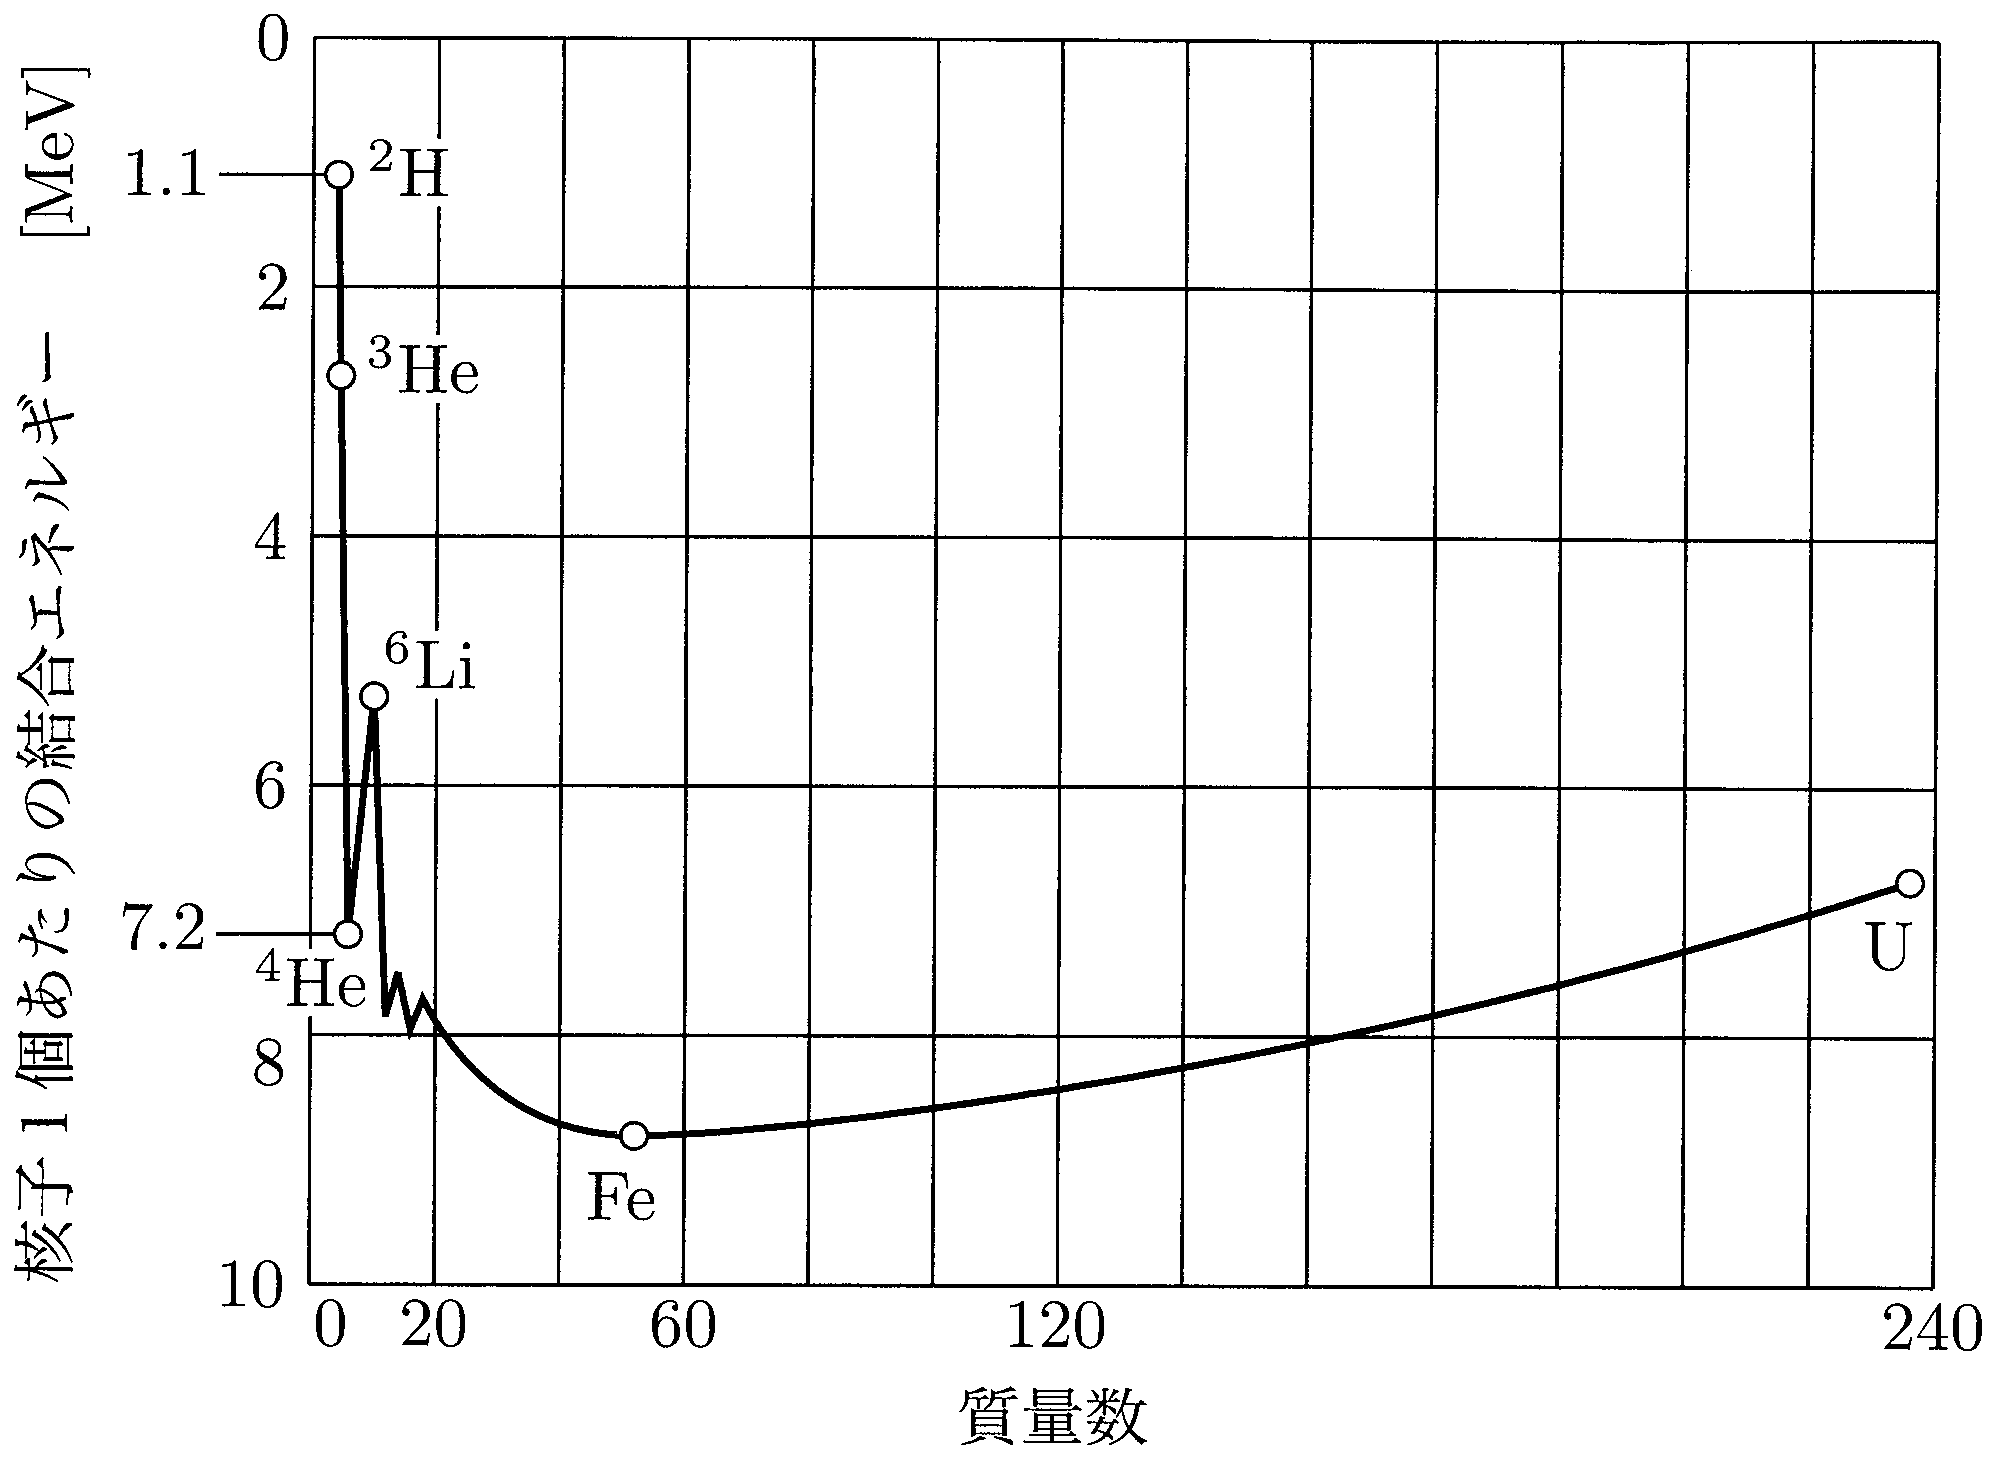
\includegraphics[keepaspectratio,width=68mm]{fig/n34_p17_zu.png}
\end{zuright}
\hspace{1zw}上図は種々の原子核について得られた核子1個あたりの平均結合エネルギーと質量数との関係を示したものである．縦軸の単位としては$1\U{MeV}=$\BOX{6}$\U{J}$を用いている．
\par
\hspace{1zw}一般に核子1個あたりの平均結合エネルギーが大きいほど，原子核は安定であると考えられる．上図から${}^2_1\mathrm{H}$より${}^3_2\mathrm{He}$が安定，${}^4_2\mathrm{He}$は${}^2_1\mathrm{H}$や${}^3_2\mathrm{He}$よりかなり安定であることがわかる．このように軽い原子核にあっては一般に質量数の大きい方が安定であるという傾向が見られる．このことは以下のようなことからも確かめられる．
\par
\hspace{1zw}ある条件下（加速器による実験や太陽の中心のような超高温状態など）においては軽い原子核同士が衝突してより質量数の大きい原子核が生成され，余った結合エネルギーが放出される反応（原子核反応）が起こる．例えば重水素${}^2_1\mathrm{H}$ 2個が衝突して三重水素${}^3_1\mathrm{H}$ 1個と水素${}^1_1\mathrm{H}$ 1個が生成され，その際$4.0\U{MeV}$のエネルギーが放出される次のような原子核反応式がある．
\[{}^2_1\mathrm{H}+{}^2_1\mathrm{H}\to{}^3_1\mathrm{H}+{}^1_1\mathrm{H}+4.0\U{MeV}\quad\cdots\cdots\text{\MARU{1}}\]
\hspace{1zw}このような原子核反応においては，電荷の保存則や，質量エネルギーを含めたエネルギー保存則が成り立つ．図から得られる${}^2_1\mathrm{H}$の結合エネルギーと\MARU{1}式から${}^3_1\mathrm{H}$の核子1個あたりの平均結合エネルギーを求めると，\BOX{7}$\U{MeV}$となる．同様に重水素と三重水素が衝突して${}^4_2\mathrm{He}$ができる反応式は
% 原本はこの式の番号も「①」（②の誤り）．
\[{}^2_1\mathrm{H}+{}^3_1\mathrm{H}\to{}^4_2\mathrm{He}+{}^1_0\mathrm{n}+\text{\BOX{8}}\U{MeV}\quad\cdots\cdots\text{\MARU{2}}\]
となる．

\Mon[\Sitei]{炭素14による年代測定}

\hspace{1zw}以下は炭素${}^{14}_{\ 6}\mathrm{C}$を用いた年代測定に関する文章である．空欄\BOX{1}〜\BOX{5}に適当な語句・数値を埋めよ．アボガドロ数は$N_{\mathrm{A}}=6.0\times 10^{23}\U{/mol}$，$\sqrt{2}=1.4$とし，数値は有効数字2桁で答えよ．
\par
\hspace{1zw}宇宙線と大気との原子核反応で生じた中性子は，大気中の窒素に吸収され，\MARU{1}式のように中性子を\BOX{1}個含む炭素をつくる．
\[{}^{14}_{\ 7}\mathrm{N}+{}^1_0\mathrm{n}\to{}^{14}_{\ 6}\mathrm{C}+{}^1_1\mathrm{p}\quad\cdots\cdots\text{\MARU{1}}\]
${}^{14}_{\ 6}\mathrm{C}$は天然の炭素の大部分を占める${}^{12}_{\ 6}\mathrm{C}$の\BOX{2}であり，半減期5700年で\MARU{2}のように\BOX{3}崩壊する．
\[{}^{14}_{\ 6}\mathrm{C}\to{}^{14}_{\ 7}\mathrm{N}+{}^{\ \ 0}_{-1}\mathrm{e}\quad\cdots\cdots\text{\MARU{2}}\]
\hspace{1zw}${}^{14}_{\ 6}\mathrm{C}$は\MARU{2}式に従って崩壊するが，大気中においては宇宙から降り注ぐ宇宙線により大気圏の上層で常に生成されるため，大気中の${}^{14}_{\ 6}\mathrm{C}$の同位体存在比は過去数千年間一定であることが知られている．植物は炭酸同化作用により${}^{14}_{\ 6}\mathrm{C}$と${}^{12}_{\ 6}\mathrm{C}$を同時に植物内に取り込むため，植物が生きている間は植物内の${}^{14}_{\ 6}\mathrm{C}$の存在比は大気中のそれとほぼ同一のまま保たれるが，植物が枯れると二酸化炭素の取り込みがなくなり，植物内の${}^{14}_{\ 6}\mathrm{C}$の存在比は減少するのみとなる．したがって，例えばある古墳から発掘された木炭中にある炭素に占める${}^{14}_{\ 6}\mathrm{C}$の割合が大気中での割合の\BOX{4}倍であったとすれば，この木炭は今から2850年前のものと推定される．
\par
\hspace{1zw}さて，大気中から分離した二酸化炭素では，\MARU{2}式の崩壊は，標準状態$1\U{L}=10^{-3}\U{m^3}$につき，1時間に約400回起こっていることが知られている．このことから大気中の単位体積$1\U{m^3}$あたりの${}^{14}_{\ 6}\mathrm{C}$の物質量は，約\BOX{5}であることがわかる．（$x$が正で1より十分小さい場合には，近似式$1-\bigl(\frac{1}{2}\bigr)^x\fallingdotseq\log_e 2\cdot x\fallingdotseq 0.70x$が成り立つことを利用して求めよ．）

\filbreak
\Rank{C問題}

\Mon{物質波の波長}

\begin{zuright}{56mm}
\hspace{1zw}現在ではすでに物質波の波長の式は分かっているが，X線の干渉実験を用いて，物質波の波長がどのような式で与えられるかを求めてみよう．右図のように結晶内のある原子面に対し入射角$\theta$でX線を入射させる．この原子面に対して垂直な方向を$z$軸にとる．プランク定数を$h\U{J\cdot s}$として以下の設問に答えよ．ただし，光子の運動量の式$p=\dfrac{h}{\lambda}$は既知としてよい．
\zusep
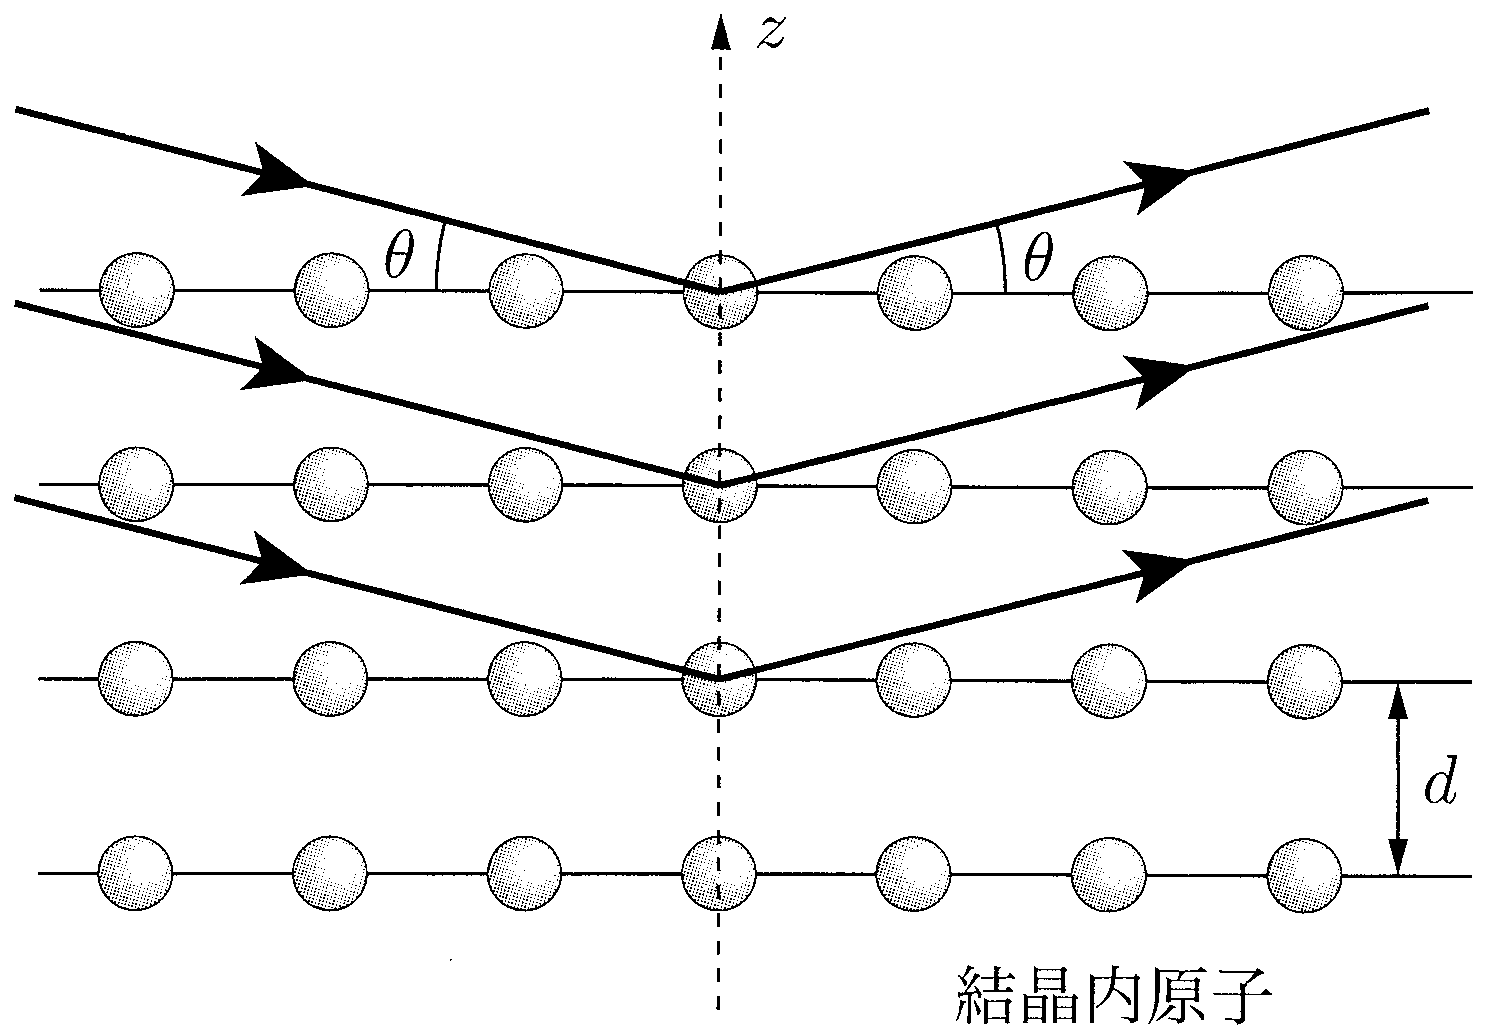
\includegraphics[keepaspectratio,width=54mm]{fig/n34_p19_zu.png}
\end{zuright}
\begin{komon}
\ko{1} X線の波長を$\lambda\U{m}$として，隣り合う面で反射されたX線が干渉し，強め合う条件（ブラッグの反射条件）を自然数$n$を用いて示せ．
\ko{2} (1)のX線を運動量を持つ粒子（光子）と考えると，このX線の反射の現象は，X線粒子が原子面と衝突し，その運動量の$z$成分の符号のみを変えて反射したのだと考えられる．1個のX線粒子が原子面と衝突したときの$z$軸方向の運動量変化を$\Delta p\U{kg\cdot m/s}$として，(1)で与えられたブラッグの反射条件を$\Delta p$を用いて書き直せ．
\ko{3} (2)で得られた結果を結晶による物質波の反射条件とし，電子線の場合にも同じ関係式が成立するものと考えよう．今，質量$m_{\mathrm{e}}\U{kg}$，速さ$v\U{m/s}$の電子からなる電子線を図と同様に入射角$\theta$で入射させたとき，反射電子線が干渉して強め合うための条件を求めよ．ただし原子面との衝突の際，各電子は$z$軸方向の成分の符号のみを変えるものとする．
\ko{4} (3)で得られた結果と(1)で与えられたブラッグの反射条件とを比較して，電子を波動と考えたときのド・ブロイ波長$\lambda_{\mathrm{e}}\U{m}$を求めよ．
\end{komon}

\Mon{原子核反応}

% 原本の反応式は中性子を「{}^1_1n」と誤記（{}^1_0n）．
\hspace{1zw}${}^{10}_{\ 5}\mathrm{B}+{}^1_0\mathrm{n}\to{}^7_3\mathrm{Li}+{}^4_2\mathrm{He}$の式で表される原子核反応がある．この反応が静止していたホウ素${}^{10}_{\ 5}\mathrm{B}$に速度がほとんど$0\U{m/s}$の中性子${}^1_0\mathrm{n}$が衝突して起こったとして以下の設問に答えよ．ただし，${}^1_0\mathrm{n}$，${}^4_2\mathrm{He}$，${}^7_3\mathrm{Li}$，${}^{10}_{\ 5}\mathrm{B}$の質量はそれぞれ$1.00898\U{u}$，$4.00388\U{u}$，$7.01822\U{u}$，$10.01677\U{u}$である．
\begin{komon}
\ko{1} この反応で放出されるエネルギー$\Delta E\U{MeV}$を求めよ．ただし質量$1\U{u}$が$931\U{MeV}$のエネルギーに相当することを用いてよい．
\ko{2} $\mathrm{He}$と$\mathrm{Li}$の速さの比$v_{\mathrm{He}}:v_{\mathrm{Li}}$および運動エネルギーの比$E_{\mathrm{He}}:E_{\mathrm{Li}}$を，${}^4_2\mathrm{He}$，${}^7_3\mathrm{Li}$の質量$m_{\mathrm{He}}$，$m_{\mathrm{Li}}$を用いて表せ．
\ko{3} 放出されたエネルギーがすべて$\mathrm{He}$と$\mathrm{Li}$の運動エネルギーに転化されたとして，$E_{\mathrm{He}}\U{MeV}$，$E_{\mathrm{Li}}\U{MeV}$の値を求めよ．
\end{komon}

\Mon{$\alpha$粒子と原子核}

\begin{zuright}{54mm}
\hspace{1zw}以下の空欄\BOX{1}〜\BOX{5}に適当な語句および式を埋めよ．
\par
\hspace{1zw}質量$m\U{kg}$，電荷$Ze\U{C}$，運動エネルギー$E\U{J}$の$\alpha$粒子が，質量$m^\prime\U{kg}$，電荷$Z^\prime e\U{C}$の静止している金の原子核に無限遠方から近づいてきて正面衝突する場合を考える．今までは$\alpha$粒子が金の原子核に近寄っても金の原子核は動かないと近似してきたが，実際には$\alpha$粒子が原子核に近づくと，その間の静電気的斥力によって原子核は$\alpha$粒子の進行方向と同じ方向に動き出す．簡単のため，原子核の運動が一直線上で起こるものとしてこれについて考えてみよう．
\zusep
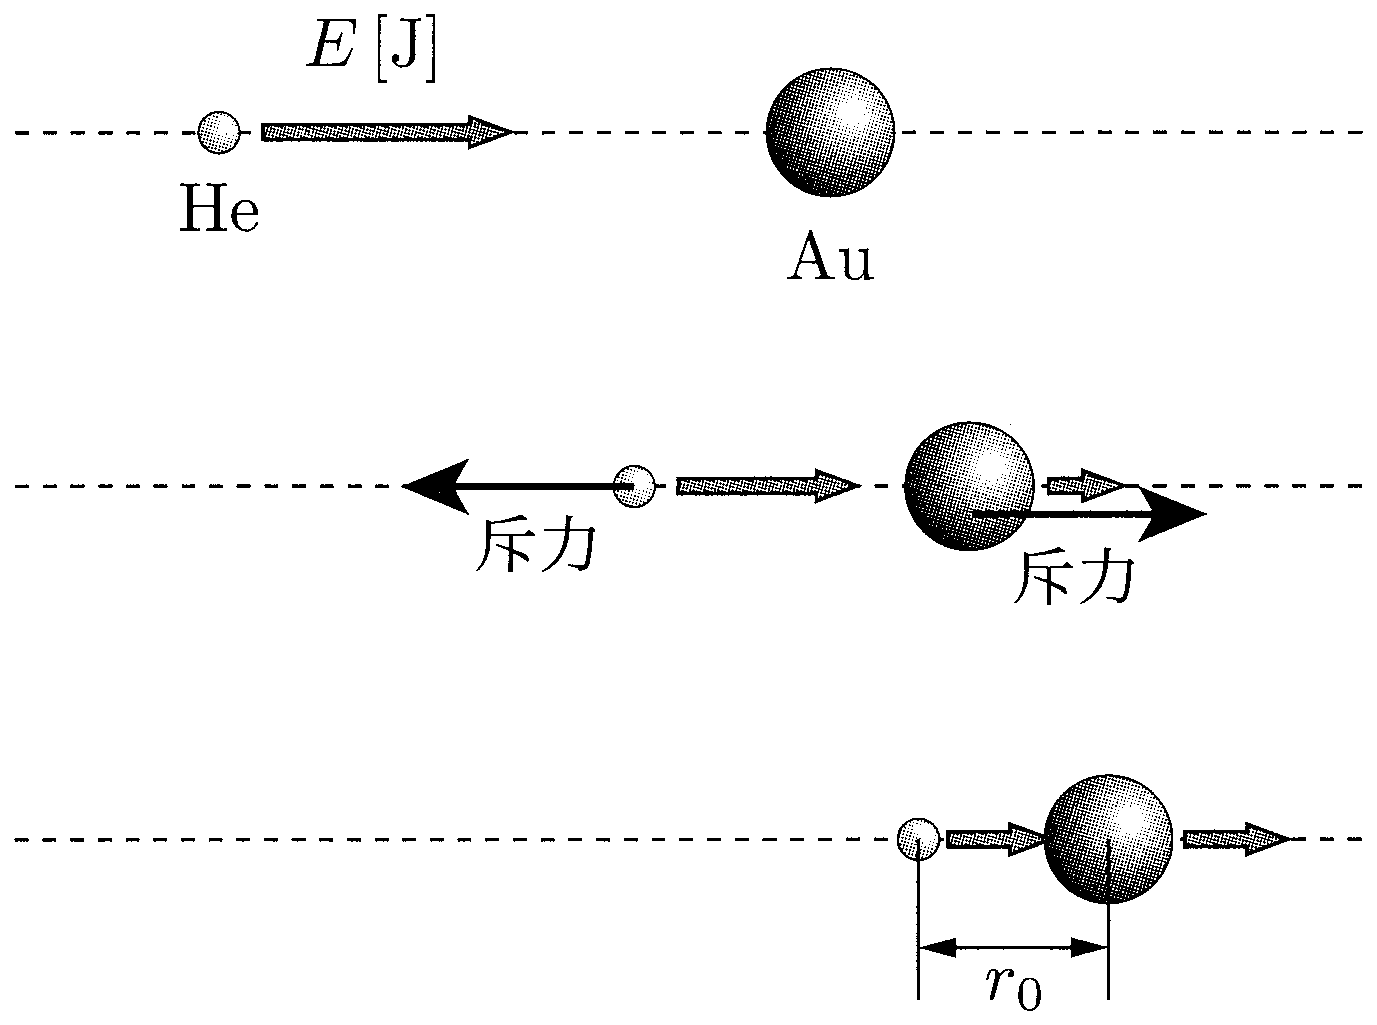
\includegraphics[keepaspectratio,width=52mm]{fig/n34_p21_zu.png}
\end{zuright}
\hspace{1zw}$\alpha$粒子が原子核に最も近づいた瞬間の原子核の速さを$v_1\U{m/s}$とすれば，$v_1=$\BOX{1}$\U{m/s}$となる．一方，原子核から距離$r\U{m}$にある$\alpha$粒子の位置エネルギーは，無限遠方を基準点にとれば，クーロンの比例定数$k_0\U{N\cdot m^2/C^2}$を用いて，\BOX{2}$\U{J}$と表せるので，$\alpha$粒子が原子核に最も近づき得る距離を$r_0\U{m}$とすれば，エネルギー保存則を適用して，$r_0=$\BOX{3}$\U{m}$となる．また$\alpha$粒子は$r_0$まで近づくと斥力で押し戻されるが，この間も原子核は加速されており，最終的には速さ$v_2=$\BOX{4}$\U{m/s}$になる．したがって跳ね返ってきた$\alpha$粒子が失ったエネルギーは\BOX{5}$\times E\U{J}$となる．

\Mon{質量とエネルギー}

\begin{zuright}{50mm}
\hspace{1zw}以下の空欄\BOX{1}〜\BOX{10}に適当な語句および式を埋めよ．
\par
\hspace{1zw}質量$m\U{kg}$，速さ$v\U{m/s}$の粒子の運動エネルギーを$K\U{J}$とする．ここで，この粒子の運動量の大きさ$p\U{kg\cdot m/s}$を$m$，$K$を用いて表すと$p=$\BOX{1}となる．しかし光子の場合には，エネルギー$E\U{J}$と運動量$p$の関係は粒子の場合とは異なり，運動量の大きさは光速$c\U{m/s}$を用いて，$p=$\BOX{2}となる．
\par
\hspace{1zw}この点に留意して以下の考察を行い，エネルギーと質量の関係を求めてみよう．図1のように質量$M\U{kg}$の静止物体から振動数$\nu\U{Hz}$の光子が2個，互いに逆向きに（同時に）放出されて，質量が$M^\prime\U{kg}$になったとする．
\zusep
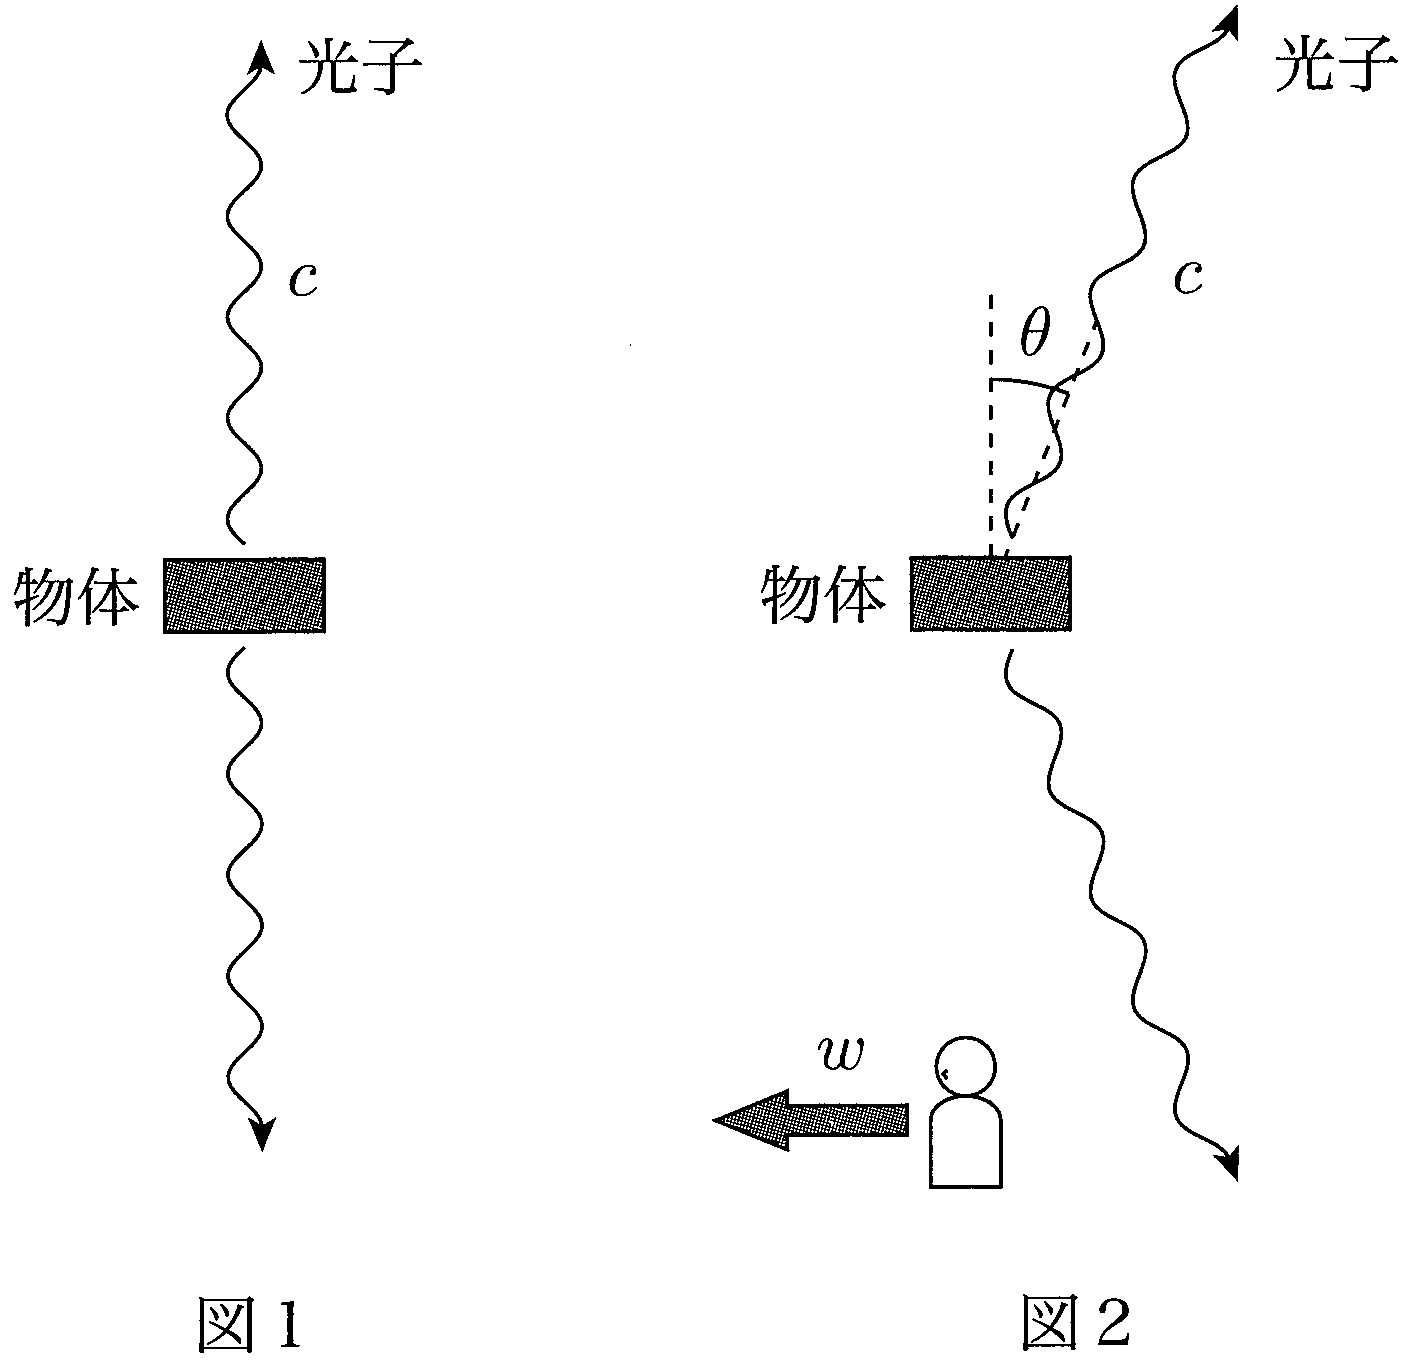
\includegraphics[keepaspectratio,width=48mm]{fig/n34_p22_zu.png}
\end{zuright}
プランク定数を$h\U{J\cdot s}$とすれば，それぞれの光子の運動量の大きさは，\BOX{3}$\U{kg\cdot m/s}$と表され，2つの光子の運動量のベクトル和は\BOX{4}であるから光子放出後の物体の速さは\BOX{5}$\U{m/s}$となる．
\par
\hspace{1zw}これを図2のように，光子の運動方向と垂直な向きに速さ$w\U{m/s}$で動いている観測者から見てみると，光子は物体の運動方向と垂直にではなく，垂直方向から$\theta$だけ傾いた方向に出ていくように見える．$w$が$c$に比べて十分小さければ，この観測者からでも振動数は$\nu$のままとしてよく，また光子の放出前後の質量もそれぞれ図1の観測者で見たものと同じ$M$，$M^\prime$のままでよいので，運動量保存則より，$Mw=$\BOX{6}となる．相対性原理によれば，光の速さはどのような系から見ても不変であることが知られているので，図2のような場合でも観測者からは光速は$c$に見える．そのため$\sin\theta$は$c$，$w$を用いて$\sin\theta=$\BOX{7}と表せるから，$(M-M^\prime)w=$\BOX{8}となる．この式は，物体の質量が\BOX{9}だけ減ったことを表す．これは放出された2個の光子のエネルギーの和$\Delta E\ (=E)\U{J}$と質量の減少分$\Delta M=M-M^\prime\U{kg}$との間に$\Delta E=$\BOX{10}の関係があることを示している．

\newpage

%%%%%%%%%%%%%%%%%%%%  解答  %%%%%%%%%%%%%%%%%%%%
\KaiTitle{第34回　X線・原子核と原子核反応}
\setlength{\columnseprule}{0.4pt}
\begin{multicols}{2}
\raggedcolumns

\Rank{A問題}
\MonN{10}{基本事項の確認}\par\nopagebreak
\begin{sisin}
原子物理は，暗記する事項が多いのだが，しっかり覚えてさえいれば解ける問題がほとんどである．面倒くさがらず，きちんと暗記してしまおう．知識としては化学とダブる部分もかなり多いはずである．
$1\U{u}\fallingdotseq 931\U{MeV}$は暗記しておこう．
(3)については，原子番号＝電気量とみなして処理するが，${}^1_0\mathrm{n}$，${}^{\ \ 0}_{-1}\mathrm{e}^-$の書き方からもすぐに分かるはず．
\end{sisin}
\KaiHead
\begin{komon}
\ko{1} ア：原子核\quad イ：電子\quad ウ：陽子\quad エ：中性子\quad オ：原子番号\quad カ：質量数\quad キ：同位体\Ans
\ko{2} 質量数35の塩素原子の存在率を$\alpha$とすると
% 原本は右辺を「33.5」と誤記（原子量35.5）．
       \[35\alpha+37(1-\alpha)=35.5\quad\Leftrightarrow\quad\alpha=0.75\]
       よって\quad $75\%$\Ans
\ko{3} 中性子は$0$，電子は$-1$\Ans
\ko{4} \[\begin{aligned}E&=mc^2=1.0\times 10^3\times(3.0\times 10^8)^2\\&=9.0\times 10^{19}\U{J}\end{aligned}\]
       \hspace*{\fill}$\cdots$(答)
\ko{5} 3時間後には，半分になるのを3回繰り返しているので$\Bigl(\dfrac{1}{2}\Bigr)^3=\dfrac{1}{8}$倍．\Ans\par
       また$\dfrac{1}{1024}=\Bigl(\dfrac{1}{2}\Bigr)^{10}$であるから，半分になるのを10回繰り返せばよい．よって\quad 10時間後\Ans
\ko{6} 陽子の質量はおよそ$1\U{u}$である．${}^{12}_{\ 6}\mathrm{C}$の1原子の質量が$12\U{u}$であることから，陽子の質量は
       \[\begin{aligned}&\frac{12\times 10^{-3}\U{kg/mol}}{6.02\times 10^{23}\U{/mol}}\times\frac{1}{12}\\&\fallingdotseq 1.66\times 10^{-27}\U{kg}\end{aligned}\]
       \hspace*{\fill}$\cdots$(答)
       また，これは
       \[\begin{aligned}&1.66\times 10^{-27}\times(3.0\times 10^8)^2\\&\fallingdotseq 1.49\times 10^{-10}\U{J}\\&=\frac{1.49\times 10^{-10}}{1.6\times 10^{-19}}\U{eV}\fallingdotseq 9.3\times 10^2\U{MeV}\end{aligned}\]
       のエネルギーに相当する．\Ans
\end{komon}

\Rank{B問題}
\MonN{11}{X線の発生機構}\par\nopagebreak
\begin{sisin}
特性X線の発生機構について問う問題である．連続X線については，衝突した電子の運動エネルギーがX線のエネルギーとターゲットの熱エネルギーに分配されることにより生じるが，特性X線については題意にあるように，電子がターゲット物質内の内殻電子をはじき出すことにより発生する．すなわち，内殻電子をはじき出すとその軌道へと上の軌道から電子が落ちてきて，その遷移に対応する光子が放出される．これが特性X線である．電子遷移により失われるエネルギーの大きさはターゲット物質のエネルギー準位により決まるため，特性X線の波長はターゲット物質の種類ごとに異なるわけである（34.1）．
\end{sisin}
\KaiHead
\begin{komon}
\ko{1} 連続\Ans
\ko{2} 特性（固有）\Ans
\ko{3} 運動エネルギー\Ans
\ko{4} 衝突直前に持つ運動エネルギーは$eV$であるから，エネルギー保存則より$eV=\dfrac{hc}{\lambda_{\min}}$．よって
       \[\lambda_{\min}=\frac{hc}{eV}\U{m}\Ans\]
\ko{5} 電子遷移により失われるエネルギーは$E_1-E_2$であり，これに相当するエネルギーの光子が放出されるので$\dfrac{hc}{\lambda_0}=E_1-E_2$．これを解いて
       \[\lambda_0=\frac{hc}{E_1-E_2}\U{m}\Ans\]
\end{komon}
\begin{bsHosoku}{参考}
特性X線，連続X線の発生機構の違いから，それぞれについて以下の性質が得られる．
\MARU{1}\ X線の強度はターゲットに当たる電子数に比例する．
\MARU{2}\ 連続X線の最短波長は電子の加速電圧（電子の運動エネルギー）にのみ依存する．
\MARU{3}\ 特性X線の波長は電子の加速電圧に依存しない．
\end{bsHosoku}

\MonN[\Sitei]{12}{ブラッグ反射条件・物質波}\par\nopagebreak
\begin{sisin}
加速電圧が$V$のときの電子線の波長の式$\lambda=\dfrac{h}{\sqrt{2m_{\mathrm{e}}eV}}$はすぐに求められるように練習しておくこと（第33回の例題5）．
ブラッグの反射条件式$2d\sin\theta=n\lambda$を利用するだけの問題なので簡単だろう．問題は(4)．結論としては，$\mathrm{A^\prime}$，$\mathrm{B^\prime}$，$\mathrm{C^\prime}\cdots$の面間隔$\dfrac{d}{\sqrt{2}}$を利用してブラッグの反射条件式を立てればよいのだが，なぜそうなるのかをきちんと考えてみよう．
\end{sisin}
\KaiHead
\begin{komon}
\ko{1} 加速後の電子の速さを$v$とすると，$\dfrac{1}{2}m_{\mathrm{e}}v^2=eV$より$v=\sqrt{\dfrac{2eV}{m_{\mathrm{e}}}}$．ド・ブロイの関係$\lambda=\dfrac{h}{m_{\mathrm{e}}v}$より
       \[\lambda=\frac{h}{\sqrt{2m_{\mathrm{e}}eV}}\U{m}\Ans\]
\ko{2} 原子配列面$\mathrm{A}$，$\mathrm{B}$，$\mathrm{C}\cdots$の面間隔は$d$であるから，ブラッグの反射条件式より
       \[2d\sin\theta=n\lambda\Ans\]
\ko{3} 以上2式から$\lambda$を消去し，$V$について解くと
       \[V=\frac{n^2h^2}{8m_{\mathrm{e}}ed^2\sin^2\theta}\U{V}\Ans\]
\ko{4} 原子面$\mathrm{A^\prime}$，$\mathrm{B^\prime}$，$\mathrm{C^\prime}\cdots$で散乱された反射電子線が強め合うか否かを判定するために，下図のように入射・反射電子線から垂線を降ろし，$\mathrm{E}\sim\mathrm{H}$と各点を名付ける．
       \begin{center}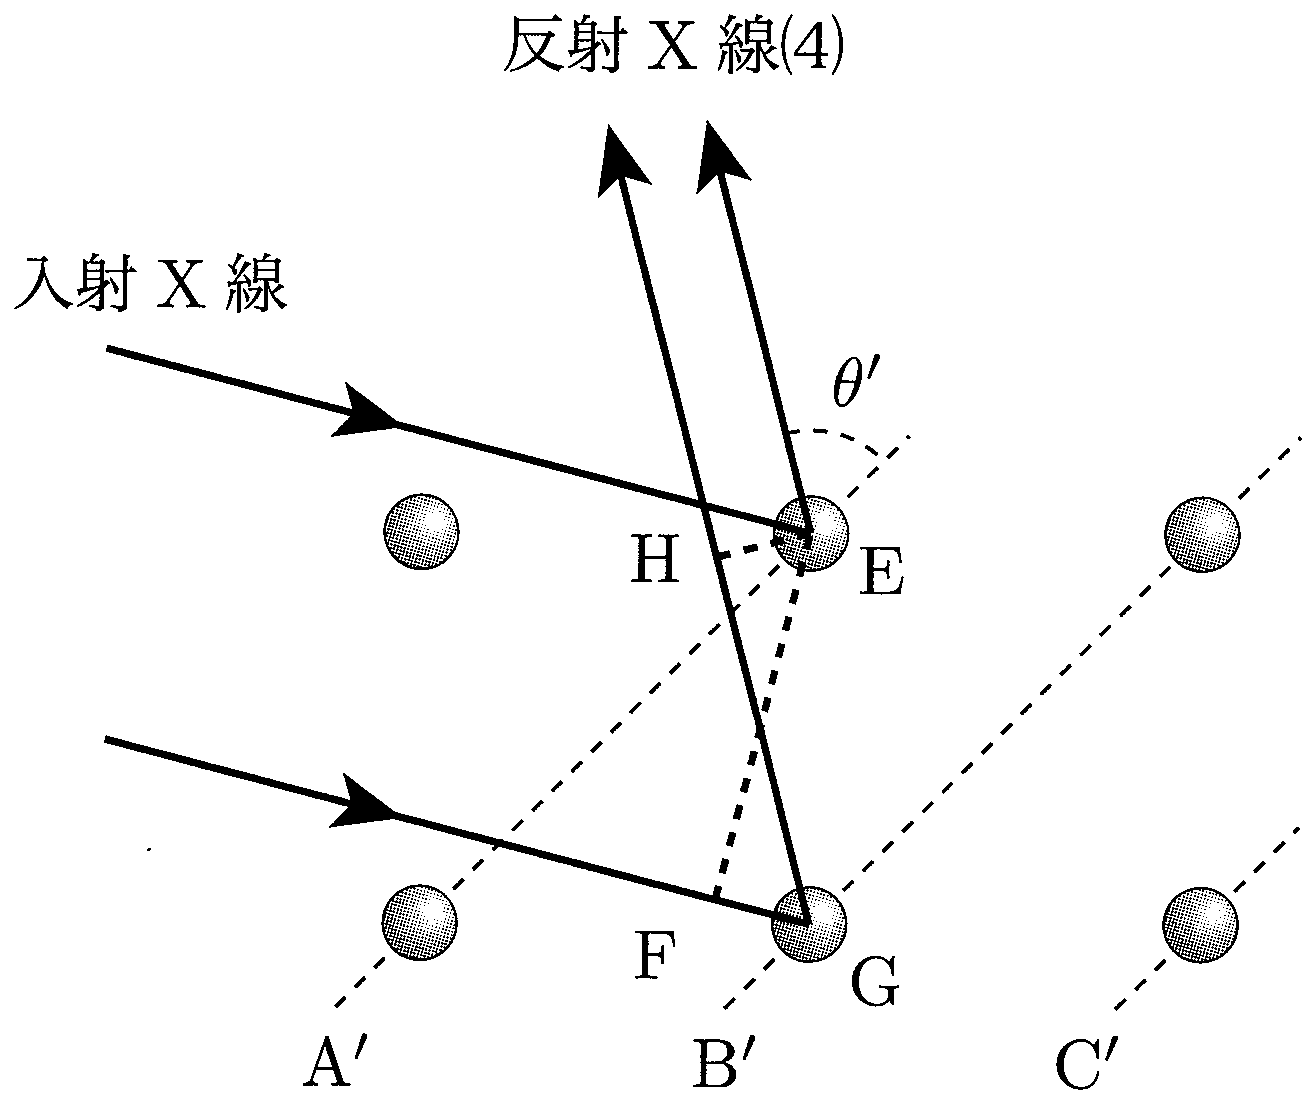
\includegraphics[keepaspectratio,width=44mm]{fig/n34_a12_zu.png}\end{center}
       このとき，隣り合う入射電子線は$\mathrm{E}$，$\mathrm{F}$で位相が揃っているので，反射電子線が強め合うためには$\mathrm{F}\sim\mathrm{G}\sim\mathrm{H}$の区間が整数波長になっていて，$\mathrm{E}$，$\mathrm{H}$で位相が揃っていればよい（下側の入射電子線の方が$\mathrm{F}\sim\mathrm{G}\sim\mathrm{H}$の区間の分だけ余計に回ってくる）．ここで
       \[\overline{\mathrm{FG}}=d\sin\theta,\qquad\overline{\mathrm{GH}}=d\cos\theta\]
       であるから$\overline{\mathrm{FG}}+\overline{\mathrm{GH}}=\sqrt{2}d\sin(\theta+45^\circ)$である．以上より，強め合うための条件は$\sqrt{2}d\sin(\theta+45^\circ)=n\lambda$であり，$\theta^\prime$を用いて表すと
       \[\sqrt{2}d\sin\theta^\prime=n\lambda\Ans\]
       \begin{bsHosoku}{参考}
       得られた答を変形すると$2\cdot\dfrac{d}{\sqrt{2}}\sin\theta^\prime=n\lambda$となり，これは面間隔が$\dfrac{d}{\sqrt{2}}$の場合のブラッグの反射条件式である．つまり，この問題のように傾いた原子面で散乱される場合についても，単純にその面間隔をとってブラッグの反射条件式を立ててやればよい．
       \end{bsHosoku}
\end{komon}

\MonN[\Sitei]{13}{放射壊変}\par\nopagebreak
\begin{sisin}
放射壊変のまとめ問題であるが，各壊変で放出される粒子の表式をしっかり覚えておきさえすれば簡単．$\alpha$崩壊はヘリウムの原子核${}^4_2\mathrm{He}^{2+}$を放出，$\beta$崩壊は電子${}^{\ \ 0}_{-1}\mathrm{e}^-$を放出，$\gamma$崩壊は光子（電磁波）を放出する．崩壊の反応式を書き，壊変前後の全質量数（左上の数の和）および全陽子数（左下の数の和）の保存を考えればよい．
% 原本は「全質量数（左下の数の和）」（左上の誤り）．
なお$\gamma$崩壊は原子核の状態遷移（核異性体転移）である．$\alpha$，$\beta$崩壊のように原子核の一部が分裂するのではないことに注意．また，このとき放出される$\gamma$線はX線などと同じく光子であるが，X線などに比べて非常に大きなエネルギーを持つ光子である．
電離作用の大小関係$\gamma<\beta<\alpha$，透過力の大小関係$\alpha<\beta\ll\gamma$も併せて覚えておくとよい．電離作用と透過力はおおよそ裏返しの関係になる（物質内の電子と相互作用しなければ透過力は当然大きくなるため）．
\end{sisin}
\KaiHead
\begin{komon}
\ko{1} ヘリウムの原子核${}^4_2\mathrm{He}^{2+}$\Ans
\ko{2} $2$\Ans
\ko{3} $4$\Ans
\ko{4} 電子${}^{\ \ 0}_{-1}\mathrm{e}^-$\Ans
\ko{5} $1$\Ans
\ko{6} 光子（電磁波）\Ans
\ko{7} 核外電子の遷移\Ans
\ko{8} 原子核\Ans
\ko{9} $\alpha$線\Ans
\ko{10} $\gamma$線\Ans
\end{komon}
\begin{bsHosoku}{参考}
$\alpha$線・$\beta$線・$\gamma$線を区別するには，電場・磁場に対する曲がり方の違いを調べればよい．$\gamma$線は光子であるから電場・磁場によって進行方向が曲げられない．$\alpha$線と$\beta$線は荷電粒子であるから電場・磁場によって進行方向が曲げられ，さらに電荷の正負が違うので，曲げられる方向が違う．
\end{bsHosoku}

\MonN{14}{放射壊変の回数}\par\nopagebreak
\begin{sisin}
放射壊変は，壊変の反応式を書き下して，原子核反応式と同様に，\MARU{1}全陽子数，\MARU{2}全質量数の保存を考えればよい（例題10）．
$\alpha$崩壊では質量数は4ずつ変化，$\beta$崩壊・$\gamma$崩壊では質量数は変化しない．そのため，放射壊変では質量数は4ずつしか変化しない．よって，質量数を4で割った余りの数で分類して，ウラン系列，アクチニウム系列，トリウム系列，ネプツニウム系列といった名称が付けられている（34.5）．
\end{sisin}
\KaiHead
\begin{komon}
\ko{1} 放射壊変では質量数は4ずつしか変化しないので，${}^{226}_{\ 88}\mathrm{Ra}$の質量数の変化は$226\to 222\to 218\to 214\to 210\to 206\to\cdots$としかならず，$204$，$205$，$207$になることはない．よって
       \[206\Ans\]
\ko{2} $\alpha$崩壊を$x$回，$\beta$崩壊を$y$回行ったとすると，反応式は
       \[{}^{226}_{\ 88}\mathrm{Ra}\to{}^{206}_{\ 82}\mathrm{Pb}+x\,{}^4_2\mathrm{He}+y\,{}^{\ \ 0}_{-1}\mathrm{e}\]
       全質量数・全陽子数の保存より$226=206+4x$，$88=82+2x-y$．これを解いて$(x,y)=(5,4)$．よって
       \[\alpha\text{崩壊：}5\text{回},\qquad\beta\text{崩壊：}4\text{回}\Ans\]
\end{komon}

\MonN{15}{半減期}\par\nopagebreak
\begin{sisin}
半減期については「今現在に存在する量が半分になるのに要する時間」と覚え，半減期の問題については「半分になるのを何回繰り返せばよいか」「半分になるのを何回繰り返して現在の量になったか」を考えよ．このことをそのまま数式においてやれば式は暗記していなくとも簡単に立てられるはずである．すなわち，半減期が$T$の物質について，時間$t$後の残存量$N$と現在の量$N_0$の間には$N=\Bigl(\dfrac{1}{2}\Bigr)^{\frac{t}{T}}N_0$が成立する．
\end{sisin}
\KaiHead
\begin{komon}
\ko{1} $12\U{s}$後における最初の物質の残存量は$1-\dfrac{7}{8}=\dfrac{1}{8}=\Bigl(\dfrac{1}{2}\Bigr)^3$であるから，$12\U{s}$後までに半分になることを3回繰り返していることが分かる．以上より
       \[T=\frac{12}{3}=4\U{s}\Ans\]
\ko{2} 要する時間を$t$とすると$\Bigl(\dfrac{1}{2}\Bigr)^{\frac{t}{T}}=\dfrac{2}{3}$が成立する．両辺の常用対数をとると
       \[-\frac{t}{T}\log_{10}2=\log_{10}2-\log_{10}3\]
       \[t=\Bigl(\frac{\log_{10}3}{\log_{10}2}-1\Bigr)T\]
       値を代入して
% 原本は「t＝0.60T＝2.4[s]」．0.4771/0.3010−1＝0.585 なので 0.585T≒2.3 s．
       \[t\fallingdotseq 0.585T\fallingdotseq 2.3\U{s}\Ans\]
\end{komon}

\MonN{16}{原子核反応式}\par\nopagebreak
\begin{sisin}
原子核反応では，\MARU{1}全陽子数，\MARU{2}全質量数，\MARU{3}全運動量，\MARU{4}全エネルギーが保存するが，特に反応式を考える場合には\MARU{1}\MARU{2}を利用する．反応式で考えれば，単純に左上，左下の数の和をそろえればよいだけであるから考えやすいだろう．
なお，(4)についてそれを行うと，質量数0，電荷$+1$の粒子が発生したことになるが，これは電子の反粒子である{\gtfamily 陽電子}である（34.8）．陽電子は質量が電子と等しく，電荷が$+e$であるような粒子であり，${}^0_1\mathrm{e}^+$だと考えればよい．
また，原子核反応式については各粒子の持つ電荷は省略して記述してよい．例えば陽子は本来${}^1_1\mathrm{p}^+$と書くのが厳密であるが，${}^1_1\mathrm{p}$と書いてもよい（ただし，電子については陽電子と通常の電子を区別するために符号をつけるのが普通である）．
\end{sisin}
\KaiHead
各原子核反応について，反応前後の全陽子数と全質量数の保存を考える．
\begin{komon}
\ko{1} 陽子数$(4+2)-6=0$，質量数$(9+4)-12=1$の粒子，すなわち中性子${}^1_0\mathrm{n}$が入る．
       \[{}^9_4\mathrm{Be}+{}^4_2\mathrm{He}\to{}^{12}_{\ 6}\mathrm{C}+{}^1_0\mathrm{n}\Ans\]
\ko{2} 陽子数$(7+2)-8=1$，質量数$(14+4)-17=1$の粒子，すなわち陽子${}^1_1\mathrm{p}$が入る．
       \[{}^{14}_{\ 7}\mathrm{N}+{}^4_2\mathrm{He}\to{}^{17}_{\ 8}\mathrm{O}+{}^1_1\mathrm{p}\Ans\]
\ko{3} 陽子数$81-82=-1$，質量数$206-206=0$の粒子，すなわち電子${}^{\ \ 0}_{-1}\mathrm{e}^-$が入る．
       \[{}^{206}_{\ 81}\mathrm{Tl}\to{}^{206}_{\ 82}\mathrm{Pb}+{}^{\ \ 0}_{-1}\mathrm{e}^-\Ans\]
\ko{4} 陽子数$15-14=1$，質量数$30-30=0$の粒子，すなわち陽電子${}^0_1\mathrm{e}^+$が入る．
       \[{}^{30}_{15}\mathrm{P}\to{}^{30}_{14}\mathrm{Si}+{}^0_1\mathrm{e}^+\Ans\]
\end{komon}

\MonN[\Sitei]{17}{結合エネルギー}\par\nopagebreak
\begin{sisin}
結合エネルギーとは，核子をすべてばらばらにするのに要するエネルギーであるから，結合している状態とばらばらの状態のエネルギー（質量エネルギー）の差が結合エネルギーとなる（34.7）．
またこの結合エネルギーによって，核融合や核分裂の定性的な説明をすることができる．最後の2つの設問については，結合エネルギーの定義式から数式的に押すよりも，化学のようなエネルギー図で考えるとあっさりと考えられるだろう．
\end{sisin}
\KaiHead
\begin{komon}
\ko{1} $Z$\Ans
\ko{2} $A-Z$\Ans
\ko{3} $A$\Ans
% 原本は「Zm_p＋(A−Z)m_e」（m_n の誤り）．
\ko{4} $Zm_{\mathrm{p}}+(A-Z)m_{\mathrm{n}}$\Ans
\ko{5} $\Delta m\cdot c^2$\Ans
\ko{6} $1\U{eV}=1.6\times 10^{-19}\U{J}$であるから$1\U{MeV}=10^6\U{eV}=1.6\times 10^{-13}\U{J}$\Ans
\ko{7} 各原子核の質量を${}^2_1\mathrm{H}$：$M_2$，${}^3_1\mathrm{H}$：$M_3$とおく（${}^1_1\mathrm{H}$は陽子そのものであるから質量は$m_{\mathrm{p}}$）．${}^2_1\mathrm{H}$の核子1個あたりの平均結合エネルギーが$1.1\U{MeV}$であることから
       \[(m_{\mathrm{p}}+m_{\mathrm{n}}-M_2)c^2=1.1\times 2\U{MeV}\quad\cdots\text{\MARU{3}}\]
       （核子が2個ゆえ原子核の結合エネルギーは$1.1\U{MeV}$の2倍である）．また，${}^3_1\mathrm{H}$の核子1個あたりの平均結合エネルギーを$Q\U{MeV}$とすると
       \[(m_{\mathrm{p}}+2m_{\mathrm{n}}-M_3)c^2=3Q\U{MeV}\quad\cdots\text{\MARU{4}}\]
       \MARU{1}の原子核反応における質量の減少量は$2M_2-M_3-m_{\mathrm{p}}$であり，この失われた質量に相当する分のエネルギーが放出されている．それが$4.0\U{MeV}$であるから
       \[(2M_2-M_3-m_{\mathrm{p}})c^2=4.0\U{MeV}\quad\cdots\text{\MARU{5}}\]
       \MARU{5}$+$\MARU{3}$\times 2-$\MARU{4}を作ると$0=4.0+2.2\times 2-3Q$．よって
       \[Q=2.8\U{MeV}\Ans\]
       \begin{bekkai}
       化学のようなエネルギー準位図で考えてもよい．
       \begin{center}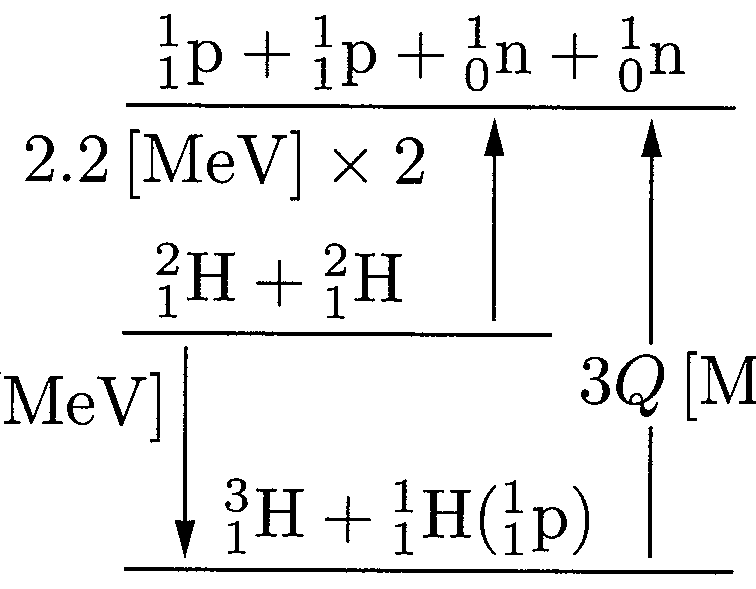
\includegraphics[keepaspectratio,width=34mm]{fig/n34_a17_lv1.png}\end{center}
       この図より$2.2\times 2+4.0=3Q$，すなわち$Q=2.8\U{MeV}$．
       \end{bekkai}
\ko{8} ${}^4_2\mathrm{He}$原子核の質量を$M_4$とおく．${}^4_2\mathrm{He}$の核子1個あたりの平均結合エネルギーが$7.2\U{MeV}$であることから
% 原本は右辺を「7.2[MeV]」と誤記（核子4個ぶんで 7.2×4）．後の計算は 7.2×4 で正しい．
       \[(2m_{\mathrm{p}}+2m_{\mathrm{n}}-M_4)c^2=7.2\times 4\U{MeV}\quad\cdots\text{\MARU{6}}\]
       \MARU{2}の原子核反応で失われる質量は$M_2+M_3-M_4-m_{\mathrm{n}}$であり，この失われた質量に相当する分のエネルギーが放出されるので，求めるべきエネルギーは$Q^\prime=(M_2+M_3-M_4-m_{\mathrm{n}})c^2$である．$-$\MARU{3}$-$\MARU{4}$+$\MARU{6}を作ると
       \[(M_2+M_3-M_4-m_{\mathrm{n}})c^2=-1.1\times 2-3Q+7.2\times 4\]
       \[Q^\prime=18.2\U{MeV}\Ans\]
       \begin{bekkai}
       ${}^4_2\mathrm{He}$原子核の結合エネルギーが$7.2\times 4=28.8\U{MeV}$であることに注意してエネルギー準位図を描くと
       \begin{center}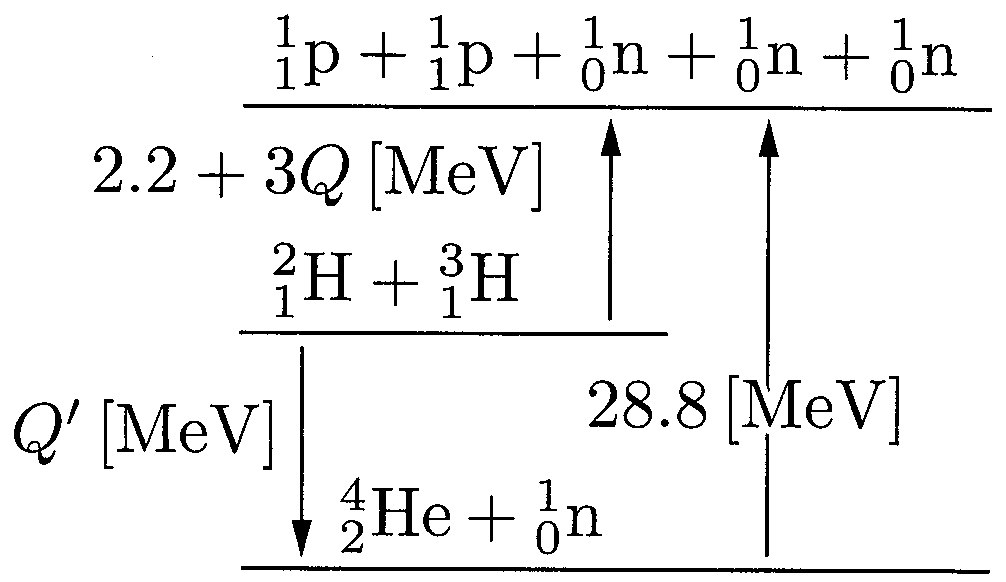
\includegraphics[keepaspectratio,width=44mm]{fig/n34_a17_lv2.png}\end{center}
       となり，$2.2+3Q+Q^\prime=28.8$より$Q^\prime=18.2\U{MeV}$．
       \end{bekkai}
\end{komon}

\MonN[\Sitei]{18}{炭素14による年代測定}\par\nopagebreak
\begin{sisin}
炭素の同位体を利用した年代測定法の原理について扱った問題である．初めて聞く内容であろうが，詳細な説明が問題文に与えてあるのだから，しっかり文章を読み取って考えよ．考え方のキーポイントは，\MARU{1}${}^{14}_{\ 6}\mathrm{C}$は植物が枯れてからは減少するのみとなるが，最初のときの${}^{14}_{\ 6}\mathrm{C}$の量（存在比）は現在の大気中における${}^{14}_{\ 6}\mathrm{C}$の量（存在比）と一致する，\MARU{2}${}^{14}_{\ 6}\mathrm{C}$の絶対量は物体の大きさなどにより変わるので${}^{14}_{\ 6}\mathrm{C}/{}^{12}_{\ 6}\mathrm{C}$の同位体存在比で考える，という2点である．
\end{sisin}
\KaiHead
\begin{komon}
\ko{1} $8$\Ans
\ko{2} 同位体\Ans
\ko{3} $\beta$\Ans
\ko{4} $2850=5700\times 0.5$であるから
       \[\Bigl(\frac{1}{2}\Bigr)^{0.5}=\frac{\sqrt{2}}{2}\fallingdotseq 0.70\ \text{倍}\Ans\]
\ko{5} 大気中$1\U{m^3}$に存在する${}^{14}_{\ 6}\mathrm{C}$の原子数を$N_0$とする．1時間は$\dfrac{1}{5700\times 365\times 24}$半減期であり，これは1より十分小さいので，1時間に崩壊する割合は与えられた近似式より
% 原本は途中式で 0.70 を落としている（数値 1.4×10^{-8} は正しい）．また 1 L あたり 400 回を 1 m^3 あたりとして立式していた．
       \[\begin{aligned}1-\Bigl(\frac{1}{2}\Bigr)^{\frac{1}{5700\times 365\times 24}}&\fallingdotseq\frac{0.70}{5700\times 365\times 24}\\&\fallingdotseq 1.4\times 10^{-8}\end{aligned}\]
       $1\U{L}=10^{-3}\U{m^3}$中で1時間に400回崩壊するので，$1\U{m^3}$中では1時間に$4.0\times 10^5$回崩壊する．よって$1.4\times 10^{-8}N_0=4.0\times 10^5$より$N_0\fallingdotseq 2.9\times 10^{13}$個．これを物質量に換算すると
       \[\frac{N_0}{N_{\mathrm{A}}}\fallingdotseq 4.8\times 10^{-11}\U{mol}\Ans\]
\end{komon}

\Rank{C問題}
\MonN{19}{物質波の波長}\par\nopagebreak
\begin{sisin}
物質波の公式$\lambda=\dfrac{h}{mv}$を導こうという趣旨の問題である．見たことのないタイプの問題であろうが，このような問題では問題文の誘導にうまく乗るように心掛けて攻めるしかない．問題文でいわんとしていることを読み取るよう，努力しよう．
\end{sisin}
\KaiHead
\begin{komon}
\ko{1} 原子面の間隔は$d$なので，ブラッグの反射条件式は
       \[2d\sin\theta=n\lambda\Ans\]
\ko{2} 衝突前後のX線粒子の運動量の$z$成分はそれぞれ$-\dfrac{h}{\lambda}\sin\theta$，$\dfrac{h}{\lambda}\sin\theta$と表せるので，$z$軸方向の運動量変化は$\Delta p=\dfrac{2h}{\lambda}\sin\theta$である．(1)と合わせて
       \[\Delta p=\frac{nh}{d}\U{kg\cdot m/s}\Ans\]
\ko{3} 衝突前後の電子の運動量の$z$成分はそれぞれ$-m_{\mathrm{e}}v\sin\theta$，$m_{\mathrm{e}}v\sin\theta$と表せるので，$\Delta p=2m_{\mathrm{e}}v\sin\theta$．これが(2)で求めたように$\dfrac{nh}{d}$となれば強め合いが起こるので，$2m_{\mathrm{e}}v\sin\theta=\dfrac{nh}{d}$．整理して
       \[2d\sin\theta=n\frac{h}{m_{\mathrm{e}}v}\Ans\]
\ko{4} この式と(1)のブラッグの反射条件式とを比較して
       \[\lambda_{\mathrm{e}}=\frac{h}{m_{\mathrm{e}}v}\U{m}\Ans\]
\end{komon}

\MonN{20}{原子核反応}\par\nopagebreak
\begin{sisin}
原子核反応では，\MARU{1}全陽子数，\MARU{2}全質量数，\MARU{3}全運動量，\MARU{4}全エネルギーが保存するが，本問は\MARU{3}\MARU{4}についても考えさせる問題である．もともとほぼ速度が$0$であるから全運動量は$0$，よって2粒子は一直線上で離れるように分かれていく．簡単な図を描きながら考えよう．
与えられた厳密な質量は，原子核反応で発生するエネルギーを求めるのに利用する．運動量保存則などを考える場合には厳密な質量を利用する必要はなく，おおまかな質量を表す質量数で近似すれば十分である（エネルギーを求めるのに質量数を使わないのは，質量数で考えると発生するエネルギーが$0$になってしまうからである．逆に$E_{\mathrm{He}}$，$E_{\mathrm{Li}}$を求めるときに厳密な質量を使っても答えはほとんど変わらない）．
\end{sisin}
\KaiHead
\begin{komon}
\ko{1} 反応前後の全質量は
       \[\text{前：}\ 10.01677+1.00898=11.02575\U{u}\]
       \[\text{後：}\ 7.01822+4.00388=11.02210\U{u}\]
       であるから，差の$0.00365\U{u}$の質量が失われ，これに相当するエネルギーが放出される．よって
       \[\Delta E=0.00365\times 931\fallingdotseq 3.40\U{MeV}\Ans\]
\ko{2} 反応前の2つの粒子がほとんど静止していたことから全運動量は$0$であり，$\mathrm{He}$と$\mathrm{Li}$は一直線上で逆向きに離れていく．運動量保存則より$0=m_{\mathrm{Li}}(-v_{\mathrm{Li}})+m_{\mathrm{He}}v_{\mathrm{He}}$であるから
       \[v_{\mathrm{He}}:v_{\mathrm{Li}}=m_{\mathrm{Li}}:m_{\mathrm{He}}\Ans\]
       また
       \[\begin{aligned}E_{\mathrm{He}}:E_{\mathrm{Li}}&=\frac{1}{2}m_{\mathrm{He}}v_{\mathrm{He}}^2:\frac{1}{2}m_{\mathrm{Li}}v_{\mathrm{Li}}^2\\&=m_{\mathrm{Li}}:m_{\mathrm{He}}\end{aligned}\]
       \hspace*{\fill}$\cdots$(答)
\ko{3} $E_{\mathrm{He}}+E_{\mathrm{Li}}=3.40\U{MeV}$，$E_{\mathrm{He}}:E_{\mathrm{Li}}=m_{\mathrm{Li}}:m_{\mathrm{He}}\fallingdotseq 7:4$であるから
       \[E_{\mathrm{He}}=3.40\times\frac{7}{11}\fallingdotseq 2.16\U{MeV}\Ans\]
       \[E_{\mathrm{Li}}=3.40\times\frac{4}{11}\fallingdotseq 1.24\U{MeV}\Ans\]
\end{komon}

\MonN{21}{$\alpha$粒子と原子核}\par\nopagebreak
\begin{sisin}
原子核反応を起こさせるためには2粒子を衝突させる必要があるが，通常，衝突させる2粒子はいずれも正電荷を持っており，電気的に反発しているので，実際に2粒子を衝突させるためにはある程度以上の運動エネルギーを持たせてやる必要がある．それを扱うのが本問である．単なる力学の問題として解けば問題ないが，注意すべき点は以下の2つである．
\MARU{1}\ 最接近したときには2粒子は同じ速さを持つ．片方の粒子の上に乗って考えれば，相手が近づいてきて最接近するとき静止して見えることから分かる．
\MARU{2}\ 位置エネルギーの式は片方の粒子のみについて考えればよい．$\alpha$粒子の持つ位置エネルギー$Ze\cdot k_0\dfrac{Z^\prime e}{r}$と金の原子核の持つ位置エネルギー$Z^\prime e\cdot k_0\dfrac{Ze}{r}$を足して系全体の位置エネルギーを$2k_0\dfrac{ZZ^\prime e^2}{r}$としてはいけない．$k_0\dfrac{ZZ^\prime e^2}{r}$の式はもともと系全体の位置エネルギーを表しているので，1つだけ考えれば十分である．
\end{sisin}
\KaiHead
\begin{komon}
\ko{1} 最初の$\alpha$粒子の速さを$v_0$とすると$E=\dfrac{1}{2}mv_0^2$より$v_0=\sqrt{\dfrac{2E}{m}}$．最初の状態と最接近した状態の間に運動量保存則を立てると$mv_0=mv_1+m^\prime v_1$．これを解いて
       \[v_1=\frac{mv_0}{m+m^\prime}=\frac{\sqrt{2mE}}{m+m^\prime}\U{m/s}\Ans\]
\ko{2} 金の原子核が距離$r$だけ離れた地点に作る電位は$k_0\dfrac{Z^\prime e}{r}$であるから，$\alpha$粒子の持つ位置エネルギーは
       \[U=Ze\cdot k_0\frac{Z^\prime e}{r}=k_0\frac{ZZ^\prime e^2}{r}\U{J}\Ans\]
\ko{3} 最初の状態と最接近したときとの間に力学的エネルギー保存則を立てると
       \[\begin{aligned}E+0&=\frac{1}{2}(m+m^\prime)v_1^2+k_0\frac{ZZ^\prime e^2}{r_0}\\&=\frac{m}{m+m^\prime}E+k_0\frac{ZZ^\prime e^2}{r_0}\end{aligned}\]
       これを解いて
% 原本は「r_0＝(m+m')/m・kZZ'e^2/E」（分母は m' が正しい）．
       \[r_0=\frac{m+m^\prime}{m^\prime}\cdot\frac{k_0ZZ^\prime e^2}{E}\U{m}\Ans\]
\ko{4} 最終的には2粒子は十分に離れる．このときの$\alpha$粒子の速度（原子核と同じ向きを正とする）を$v_3$とすると，運動量保存則と力学的エネルギー保存則より
       \[mv_0=mv_3+m^\prime v_2,\qquad E=\frac{1}{2}mv_3^2+\frac{1}{2}m^\prime v_2^2\]
       2式から$v_3$を消去して整理すると$0=-v_0v_2+\dfrac{m+m^\prime}{2m}v_2^2$．よって
       \[v_2=\frac{2mv_0}{m+m^\prime}=\frac{2\sqrt{2mE}}{m+m^\prime}\U{m/s}\Ans\]
\ko{5} (4)より$v_3=v_0-\dfrac{m^\prime}{m}v_2=\dfrac{m-m^\prime}{m+m^\prime}\sqrt{\dfrac{2E}{m}}$．以上より，$\alpha$粒子の失ったエネルギーは
       \[\begin{aligned}E-\frac{1}{2}mv_3^2&=E-\Bigl(\frac{m-m^\prime}{m+m^\prime}\Bigr)^2E\\&=\frac{4mm^\prime}{(m+m^\prime)^2}E\end{aligned}\]
       よって\quad $\dfrac{4mm^\prime}{(m+m^\prime)^2}$\Ans
\end{komon}

\MonN{22}{質量とエネルギー}\par\nopagebreak
\begin{sisin}
アインシュタインの相対性理論の式$E=mc^2$を思考実験から導こうという問題である（もちろんこれは厳密な導出ではない）．問題の誘導にうまく乗って考えること（34.7）．
\end{sisin}
\KaiHead
\begin{komon}
\ko{1} $K=\dfrac{1}{2}mv^2$，$p=mv$であるから，$v$を消去して
       \[p=\sqrt{2mK}\Ans\]
\ko{2} 光量子説より$E=\dfrac{hc}{\lambda}$，$p=\dfrac{h}{\lambda}$であるから
       \[p=\frac{E}{c}\Ans\]
\ko{3} $E=h\nu$であるから\quad $\dfrac{h\nu}{c}$\Ans
\ko{4} 光子の持つ運動量の大きさは同じで，互いに逆向きであるから\quad $\vec{0}$\Ans
\ko{5} 光子放出の前後で，系全体（物体$+$2つの光子）の運動量の和が保存される．もともと総和は$\vec{0}$であったから，光子放出後の物体の運動量は$\vec{0}$である．よって\quad $0$\Ans
\ko{6} この観測者から見ると，物体は右方向へ動いているように見え，光子も右へそれた方向へ放出されているように見える．右向きを正として運動量保存則を立てると
       \[Mw=M^\prime w+\frac{h\nu}{c}\sin\theta+\frac{h\nu}{c}\sin\theta\]
       \[Mw=M^\prime w+\frac{2h\nu}{c}\sin\theta\Ans\]
\ko{7} 速さ$w$で動く観測者から見ると，光子の放出方向は次図のようにずれる．
       \begin{center}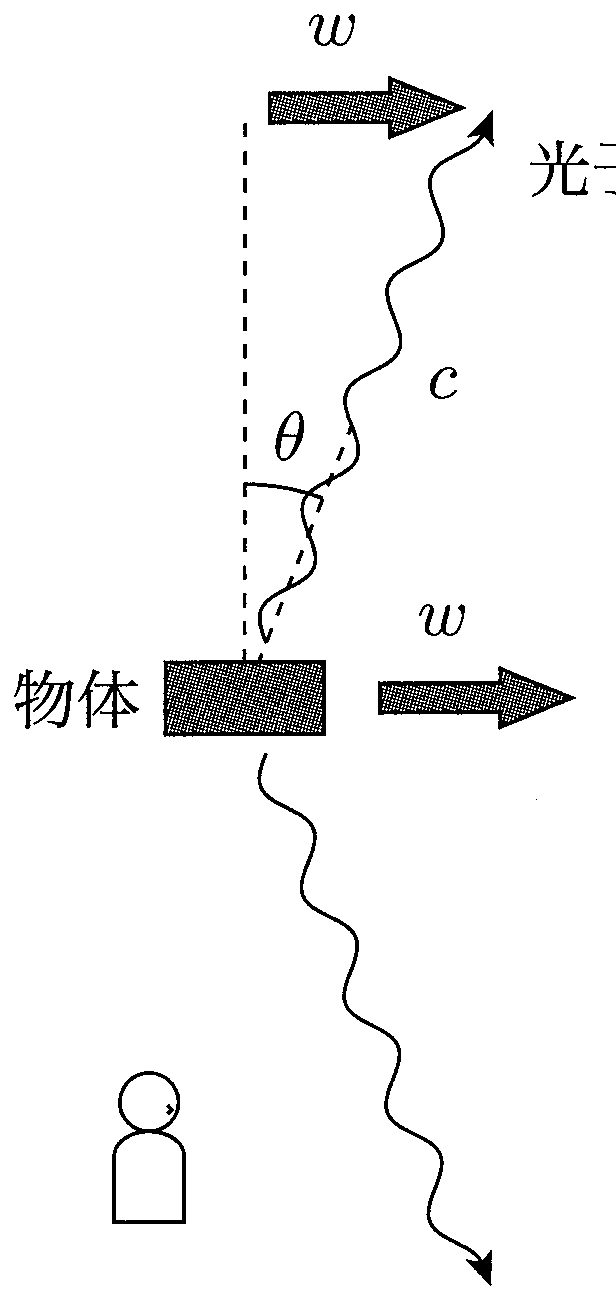
\includegraphics[keepaspectratio,width=24mm]{fig/n34_a22_zu.png}\end{center}
       光子は，速さ$c$のうち横方向に$w$の速度成分を持つように見えるので
       \[\sin\theta=\frac{w}{c}\Ans\]
\ko{8} (6)(7)より$Mw=M^\prime w+\dfrac{2h\nu}{c}\cdot\dfrac{w}{c}$となり，整理して
       \[(M-M^\prime)w=\frac{2h\nu w}{c^2}\Ans\]
\ko{9} さらに整理して，質量減少は
       \[M-M^\prime=\frac{2h\nu}{c^2}\Ans\]
\ko{10} (9)を整理すると$(M-M^\prime)c^2=2h\nu$となるが，右辺は放出された2個の光子のエネルギーの和である．すなわち
       \[\Delta E=2h\nu=\Delta M\cdot c^2\Ans\]
\end{komon}

\end{multicols}
